\chapter{曲线积分与曲面积分}

积分实际上是求连续量作用的总和．当连续量定义在直线段时，这是定积分；当连续量定义在平面的区域时，这是二重积分；当连续量定义在空间的立体时，这是三重积分．自然连续量还可以定义在空间曲线或空间曲面上，这就分别引导到曲线积分和曲面积分．定积分的积分线段是有向的，重积分的积分区域是无向的，细心的读者应看到两者的区别．定义域是无向的积分称为第一型的，定义域是有向的积分称为第二型的．因此曲线积分和曲面积分有第一型和第二型之区别，这是读者要特别注意的．

\section{第一型曲线积分与曲面积分}

上一章中，我们从求平面薄板的质量引出了二重积分，从求空间物体的质量引出了三重积分．在这里，我们将从求曲线段的质量引出第一型曲线积分，而类似地从求曲面块的质量引出第一型曲面积分．

\subsection{第一型曲线积分}

我们的问题是，设有空间的曲线段 $L$，其上每点有线密度，如何求其质量，为简单起见，设空间曲线段 $L$ 是可求长的，其端点为 $A$、$B$．又设密度函数 $f(x,y,z)$ 在曲线 $L$ 上连续，我们来求这曲线段 $L$ 的质量．

从 $A$ 至 $B$ 依次插入分点 $A=A_{0}$，$A_{1},\cdots,A_{n}=B$，它将曲线段 $L$ 分成 $n$ 小段．记第 $i$ 段弧长为 $\Delta s_{i}$ $(i=1,2,\cdots,n)$．

\begin{figure}[htbp]
\centering
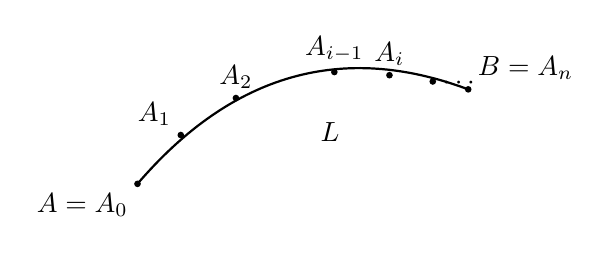
\begin{tikzpicture}[scale=1]
\draw[thick] (0,0) .. controls (1.2,1.4) and (2.6,1.8) .. (4.2,1.2);
\foreach \p/\lab in {(0,0)/$A=A_{0}$,(0.55,0.62)/$A_{1}$,(1.25,1.09)/$A_{2}$,(2.5,1.42)/$A_{i-1}$,(3.2,1.38)/$A_{i}$,(3.75,1.3)/$\cdots$,(4.2,1.2)/$B=A_{n}$}{
  \fill \p circle (1.2pt);
}
\node[below left] at (0,0) {$A=A_{0}$};
\node[above left] at (0.55,0.62) {$A_{1}$};
\node[above] at (1.25,1.09) {$A_{2}$};
\node[above] at (2.5,1.42) {$A_{i-1}$};
\node[above] at (3.2,1.38) {$A_{i}$};
\node[right] at (3.75,1.28) {$\cdots$};
\node[above right] at (4.2,1.2) {$B=A_{n}$};
\node[below right] at (2.2,0.9) {$L$};
\end{tikzpicture}\caption{\relax}\label{fig:21-1}
\end{figure}

在第 $i$ 弧段上任取一点 $(\xi_{i},\eta_{i},\zeta_{i})$，则第 $i$ 弧段的质量近似于 $f(\xi_{i},\eta_{i},\zeta_{i})\Delta s_{i}$，从而 $L$ 的质量就近似于
\[
\sum_{i=1}^{n}f(\xi_{i},\eta_{i},\zeta_{i})\Delta s_{i}.
\]
当 $\lambda=\max\limits_{1\leqslant i\leqslant n}\{\Delta s_{i}\}\to0$ 时，上述和式的极限就是 $L$ 的质量
\[
M=\lim_{\lambda\to0}\sum_{i=0}^{n}f(\xi_{i},\eta_{i},\zeta_{i})\Delta s_{i}.
\]
这种定义在曲线段 $L$ 上的和式的极限，就称为 $f(x,y,z)$ 在 $L$ 的第一型曲线积分．

一般地有下述定义．

\begin{definition}\label{def:21-1}
设 $L$ 是空间可求长的曲线段，$f(x,y,z)$ 定义在 $L$ 上．$L$ 的两端点为 $A$，$B$．依次用分点 $A=A_{0},A_{1},\cdots,A_{n}=B$ 将 $L$ 分成 $n$ 小段，每小段的弧长记为 $\Delta s_{i}$，不妨将第 $i$ 小段弧也记为 $\Delta s_{i}$．任取 $(\xi_{i},\eta_{i},\zeta_{i})\in\Delta s_{i}$，作和式
\[
\sum_{i=1}^{n}f(\xi_{i},\eta_{i},\zeta_{i})\Delta s_{i}.
\]
若当 $\lambda=\max\limits_{1\leqslant i\leqslant n}\{\Delta s_{i}\}\to0$ 时上述和式极限存在，则称此极限为 $f(x,y,z)$ 在曲线 $L$ 上的\emph{第一型曲线积分}，记为
\[
\int_{L}f(x,y,z)\,\mathrm{d}s.
\]
总起来说，就是
\[
\int_{L}f(x,y,z)\,\mathrm{d}s=\lim_{\lambda\to0}\sum_{i=1}^{n}f(\xi_{i},\eta_{i},\zeta_{i})\Delta s_{i}.
\]
\end{definition}

\begin{theorem}\label{thm:21-1}
设 $L$ 是光滑曲线
\[
x=x(t),\quad y=y(t),\quad z=z(t),\quad\alpha\leqslant t\leqslant\beta,
\]
$f(x,y,z)$ 在 $L$ 上连续，则 $f(x,y,z)$ 在 $L$ 上的第一型曲线积分存在，且
\[
\begin{aligned}
&\int_{L}f(x,y,z)\,\mathrm{d}s\\
={}&\int_{\alpha}^{\beta}f(x(t),y(t),z(t))\sqrt{x^{\prime2}(t)+y^{\prime2}(t)+z^{\prime2}(t)}\,\mathrm{d}t.
\end{aligned}
\]
\end{theorem}

\begin{proof}
（1）设 $L$ 的参数方程中的参数 $t$ 是从一端点 $A$ 到曲线上的点 $(x,y,z)$ 的弧长 $s$．这时，方程化为
\[
\begin{cases}
x=x(s),\\
y=y(s),\\
z=z(s),
\end{cases}
\quad 0\leqslant s\leqslant l,
\]
这就是曲线的本性方程．因此曲线上的分点 $A=A_{0},A_{1},\cdots,A_{n}=B$ 对应于 $[0,l]$ 的分法：$0=s_{0}<s_{1}<\cdots<s_{n}=l$．$\Delta s_{i}=s_{i}-s_{i-1}$ 既表示第 $i$ 段的弧长，也表示曲线段本身．对任意 $(\xi_{i},\eta_{i},\zeta_{i})\in\Delta s_{i}$，存在 $s_{i}^{*}\in\Delta s_{i}$，使得
\[
(\xi_{i},\eta_{i},\zeta_{i})=(x(s_{i}^{*}),y(s_{i}^{*}),z(s_{i}^{*})).
\]
因此
\[
\begin{aligned}
&\sum_{i=1}^{n}f(\xi_{i},\eta_{i},\zeta_{i})\Delta s_{i}\\
={}&\sum_{i=1}^{n}f(x(s_{i}^{*}),y(s_{i}^{*}),z(s_{i}^{*}))\Delta s_{i},
\end{aligned}
\]
它是 $f(x(s),y(s),z(s))$ 在 $[0,l]$ 的黎曼和．由于 $f(x(s),y(s),z(s))$ 在 $[0,l]$ 连续，从而可积，故有
\[
\int_{0}^{l}f(x(s),y(s),z(s))\,\mathrm{d}s=\lim_{\lambda\to0}\sum_{i=1}^{n}f(\xi_{i},\eta_{i},\zeta_{i})\Delta s_{i}.
\]
由定义~\ref{def:21-1} 即得 $f(x,y,z)$ 在 $L$ 上的第一型曲线积分存在，且
\[
\int_{L}f(x,y,z)\,\mathrm{d}s=\int_{0}^{l}f(x(s),y(s),z(s))\,\mathrm{d}s.
\]
注意当参数 $s$ 是弧长参数时，$x^{\prime2}(s)+y^{\prime2}(s)+z^{\prime2}(s)=1$，因此公式成立．

（2）设 $t$ 是任意参数．回忆本性方程的求法，对 $\widehat{AB}$ 上的任一点 $P(x(t),y(t),z(t))$，求出 $\widehat{AP}$ 的弧长
\[
s(t)=\int_{\alpha}^{t}\sqrt{x^{\prime2}(\tau)+y^{\prime2}(\tau)+z^{\prime2}(\tau)}\,\mathrm{d}\tau,\quad t\in[\alpha,\beta].
\]
由于
\[
\frac{\mathrm{d}s}{\mathrm{d}t}=\sqrt{x^{\prime2}(t)+y^{\prime2}(t)+z^{\prime2}(t)}>0,
\]
根据反函数存在定理知，函数 $s(t)$ 有反函数 $t=t(s)$，它在 $[0,l]$ 上连续可微，且 $t=\alpha$ 对应于 $s=0$，$t=\beta$ 对应于 $s=l$．这时
\[
\begin{cases}
x=x(t(s)),\\
y=y(t(s)),\\
z=z(t(s)),
\end{cases}
\quad 0\leqslant s\leqslant l
\]
是 $L$ 的本性方程．由（1）已证得
\[
\int_{L}f(x,y,z)\,\mathrm{d}s=\int_{0}^{l}f(x(t(s)),y(t(s)),z(t(s)))\,\mathrm{d}s.
\]
在等式右边作定积分的变量代换 $s=s(t)$，得
\[
\begin{aligned}
&\int_{L}f(x,y,z)\,\mathrm{d}s\\
={}&\int_{\alpha}^{\beta}f(x(t),y(t),z(t))\sqrt{x^{\prime2}(t)+y^{\prime2}(t)+z^{\prime2}(t)}\,\mathrm{d}t.
\end{aligned}
\]
公式得证．定理~\ref{thm:21-1} 证完．
\end{proof}

定理~\ref{thm:21-1} 把第一型曲线积分化成了定积分，从而给出了第一型曲线积分的计算方法．

\begin{sloppypar}
其实，这公式是很容易记忆的．它指出，在曲线积分
\[
\int_{L}f(x,y,z)\,\mathrm{d}s
\]
中，把 $L$ 的参数方程 $x=x(t)$，$y=y(t)$，$z=z(t)$ 代进去，再把弧微分 $\mathrm{d}s=\sqrt{x^{\prime2}(t)+y^{\prime2}(t)+z^{\prime2}(t)}\,\mathrm{d}t$ 也代进去，积分限 $t=\alpha$ 与 $t=\beta$，是对应于 $L$ 两个端点的参数．要特别注意的是，积分限永远是从小到大．这是因为，线积分定义中的 $\Delta s_{i}$ 是真正的弧长，永远是正的．由此可见，第一型曲线积分同 $L$ 的方向无关．也就是说，如果 $L$ 的两个端点是 $A$ 与 $B$，则 $f(x,y,z)$ 在 $L$ 的第一型曲线积分由 $A$ 积到 $B$ 等于由 $B$ 积到 $A$，可以把这写成
\[
\int_{\widehat{AB}}f(x,y,z)\,\mathrm{d}s=\int_{\widehat{BA}}f(x,y,z)\,\mathrm{d}s.
\]
因为由定理~\ref{thm:21-1}，它们都化成同一个定积分．
\end{sloppypar}

当 $L$ 是平面曲线且用 $y=\varphi(x)$，$a\leqslant x\leqslant b$ 给出时，公式化为
\[
\int_{L}f(x,y)\,\mathrm{d}s=\int_{a}^{b}f(x,\varphi(x))\sqrt{1+\varphi^{\prime2}(x)}\,\mathrm{d}x.
\]
显然，当 $f(x,y,z)=1$ 时，定理~\ref{thm:21-1} 的公式化为
\[
\int_{L}\mathrm{d}s=\int_{\alpha}^{\beta}\sqrt{x^{\prime2}(t)+y^{\prime2}(t)+z^{\prime2}(t)}\,\mathrm{d}s,
\]
这就是 $L$ 的弧长，与我们对曲线积分的直观理解一致．当 $f(x,y,z)$ 是 $L$ 的线密度函数时，$\displaystyle\int_{L}f(x,y,z)\,\mathrm{d}s$ 就是曲线 $L$ 的质量．定理~\ref{thm:21-1} 给出了它们的计算方法．

\begin{example}\label{ex:21-1-1}
设 $L$ 是椭圆 $\dfrac{x^{2}}{a^{2}}+\dfrac{y^{2}}{b^{2}}=1$ 在第一象限部分，求 $I=\displaystyle\int_{L}xy\,\mathrm{d}s$．
\end{example}

\begin{proof}[解法1]
用 $L$ 的参数方程
\[
x=a\cos\theta,\quad y=b\sin\theta,\quad 0\leqslant\theta\leqslant\frac{\pi}{2},
\]
则
\[
x^{\prime}=-a\sin\theta,\quad y^{\prime}=b\cos\theta,
\]
\[
\begin{aligned}
\mathrm{d}s&=\sqrt{x^{\prime2}+y^{\prime2}}\,\mathrm{d}\theta=\sqrt{a^{2}\sin^{2}\theta+b^{2}\cos^{2}\theta}\,\mathrm{d}\theta\\
&=\sqrt{\frac{a^{2}+b^{2}}{2}+\frac{b^{2}-a^{2}}{2}\cos2\theta}\,\mathrm{d}\theta.
\end{aligned}
\]
故
\[
\begin{aligned}
I&=\int_{L}xy\,\mathrm{d}s=\int_{0}^{\frac{\pi}{2}}ab\sin\theta\cos\theta\sqrt{\frac{a^{2}+b^{2}}{2}+\frac{b^{2}-a^{2}}{2}\cos2\theta}\,\mathrm{d}\theta\\
&=-\frac{ab}{4}\int_{0}^{\frac{\pi}{2}}\sqrt{\frac{a^{2}+b^{2}}{2}+\frac{b^{2}-a^{2}}{2}\cos2\theta}\,\mathrm{d}\cos2\theta\\
&=-\frac{ab}{3(b^{2}-a^{2})}\left(\frac{a^{2}+b^{2}}{2}+\frac{b^{2}-a^{2}}{2}\cos2\theta\right)^{\frac{3}{2}}\Bigg|_{0}^{\frac{\pi}{2}}\\
&=\frac{ab}{3}\frac{a^{2}+ab+b^{2}}{a+b}.
\end{aligned}
\]
\end{proof}

\begin{proof}[解法2]
用 $L$ 的直角坐标方程
\[
y=\frac{b}{a}\sqrt{a^{2}-x^{2}},\quad 0\leqslant x\leqslant a,
\]
则
\[
y^{\prime}=-\frac{bx}{a\sqrt{a^{2}-x^{2}}},
\]
\[
\mathrm{d}s=\sqrt{1+y^{\prime2}}\,\mathrm{d}x=\frac{1}{a}\sqrt{\frac{a^{4}-(a^{2}-b^{2})x^{2}}{a^{2}-x^{2}}}\,\mathrm{d}x.
\]
因此
\[
\begin{aligned}
I&=\int_{L}xy\,\mathrm{d}s=\int_{0}^{a}\frac{b}{a^{2}}x\sqrt{a^{4}-(a^{2}-b^{2})x^{2}}\,\mathrm{d}x\\
&=\frac{b}{3a^{2}(b^{2}-a^{2})}\left[a^{4}-(a^{2}-b^{2})x^{2}\right]^{\frac{3}{2}}\bigg|_{0}^{a}\\
&=\frac{ab}{3}\frac{a^{2}+ab+b^{2}}{a+b}.
\end{aligned}
\]
\end{proof}

\begin{example}\label{ex:21-1-2}
计算 $\displaystyle\int_{L}x^{2}\,\mathrm{d}s$，其中 $L$ 为球面 $x^{2}+y^{2}+z^{2}=a^{2}$ 被平面 $x+y+z=0$ 所截得的圆周．
\end{example}

\begin{proof}[解]
曲线 $L$ 是半径为 $a$、圆心在原点的圆周．但它的参数方程并不易写出．注意到 $L$ 关于 $x$，$y$，$z$ 的对称性，则有
\[
\int_{L}x^{2}\,\mathrm{d}s=\int_{L}y^{2}\,\mathrm{d}s=\int_{L}z^{2}\,\mathrm{d}s.
\]
因此
\[
\begin{aligned}
\int_{L}x^{2}\,\mathrm{d}s&=\frac{1}{3}\int_{L}(x^{2}+y^{2}+z^{2})\,\mathrm{d}s\\
&=\frac{a^{2}}{3}\int_{L}\mathrm{d}s=\frac{2}{3}\pi a^{3}.
\end{aligned}
\]
\end{proof}

对称性和几何意义是简化积分计算的常用技巧，读者应多多留意并灵活运用．

\begin{example}\label{ex:21-1-3}
试求一均匀半圆周（密度 $\rho=1$）对位于其中心的单位质点的引力．
\end{example}

\begin{proof}[解]
为计算方便，取半圆周为圆心在原点的上半圆周．设半径为 $R$，则 $x=R\cos\theta$，$y=R\sin\theta$，$(0\leqslant\theta\leqslant\pi)$．由对称性知引力 $\bm{F}$ 在 $x$ 轴上的投影 $F_{x}=0$，故只要计算 $\bm{F}$ 在 $y$ 轴上的投影 $F_{y}$．任取弧长微元 $\mathrm{d}s$，它对原点处单位质量的质点的引力为
\[
\mathrm{d}\bm{F}=\frac{k_{\rho}}{R^{2}}\mathrm{d}s\bm{r}_{0},
\]
其中 $k$ 是引力常数，$\bm{r}_{0}$ 是向径的单位向量．将 $\rho=1$，$\mathrm{d}s=R\mathrm{d}\theta$ 代进去，得 $\mathrm{d}\bm{F}$ 在 $y$ 轴上的投影为
\[
\mathrm{d}F_{y}=\frac{k}{R^{2}}\sin\theta\,\mathrm{d}s=\frac{k}{R}\sin\theta\,\mathrm{d}\theta.
\]
故 $F_{y}=\displaystyle\int_{0}^{\pi}\frac{k}{R}\sin\theta\,\mathrm{d}\theta=\frac{k}{R}\cos\theta\,\bigg|_{\pi}^{0}=\frac{2k}{R}$．
\end{proof}

\begin{figure}[htbp]
\centering
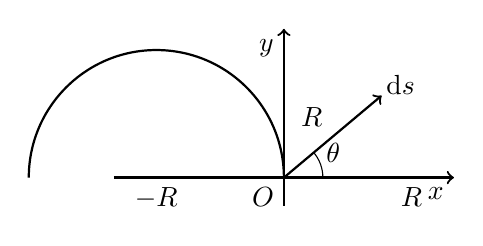
\begin{tikzpicture}[scale=0.9]
\draw[->,thick] (-2.4,0) -- (2.4,0) node[below left] {$x$};
\draw[->,thick] (0,-0.4) -- (0,2.1) node[below left] {$y$};
\draw[thick] (0,0) arc (0:180:1.8);
\draw[thick,->] (0,0) -- (40:1.8) node[midway,above left] {$R$};
\draw (0:0.55) arc (0:40:0.55) node[right,xshift=1pt] {$\theta$};
\node[below left] at (0,0) {$O$};
\node[below] at (1.8,0) {$R$};
\node[below] at (-1.8,0) {$-R$};
\node[right] at (45:1.85) {$\mathrm{d}s$};
\end{tikzpicture}\caption{\relax}\label{fig:21-2}
\end{figure}

\subsection{第一型曲面积分}

类似于第一型曲线积分，我们可以给出第一型曲面积分的定义．

\begin{definition}\label{def:21-2}
设 $S$ 是空间光滑曲面 $z=z(x,y)$，$(x,y)\in D$，$f(x,y,z)$ 是定义在 $S$ 上的函数．对于 $D$ 的任意分法 $\Delta\sigma_{i}$，相应地得到 $S$ 的分法 $\Delta S_{i}$ $(i=1,2,\cdots,n)$．任取 $(\xi_{i},\eta_{i},\zeta_{i})\in\Delta S_{i}$，记 $\lambda=\max\limits_{1\leqslant i\leqslant n}\{\Delta\sigma_{i}\ \text{的直径}\}$．若极限
\[
\lim_{\lambda\to0}\sum_{i=1}^{n}f(\xi_{i},\eta_{i},\zeta_{i})\Delta S_{i}
\]
存在，则称该极限值为 $f(x,y,z)$ 在曲面 $S$ 上的\emph{第一型曲面积分}，记为
\[
\iint_{S}f(x,y,z)\,\mathrm{d}S.
\]
\end{definition}

\begin{theorem}\label{thm:21-2}
设 $S:z=z(x,y)$，$(x,y)\in D$ 是光滑曲面，$D$ 是有界闭区域，$f(x,y,z)$ 在 $S$ 上连续，则 $f(x,y,z)$ 在曲面 $S$ 上的第一型曲面积分存在，且
\[
\begin{aligned}
&\iint_{S}f(x,y,z)\,\mathrm{d}S\\
={}&\iint_{D}f(x,y,z(x,y))\sqrt{1+z_{x}^{2}(x,y)+z_{y}^{2}(x,y)}\,\mathrm{d}x\mathrm{d}y.
\end{aligned}
\]
\end{theorem}

\begin{proof}
对于 $D$ 的任意分法 $\Delta\sigma_{i}$，相应地有 $S$ 的分法 $\Delta S_{i}$ $(i=1,2,\cdots,n)$．$\Delta S_{i}$ 的面积为
\[
\Delta S_{i}=\iint_{\Delta\sigma_{i}}\sqrt{1+z_{x}^{2}(x,y)+z_{y}^{2}(x,y)}\,\mathrm{d}x\mathrm{d}y.
\]
由二重积分的中值定理
\[
\Delta S_{i}=\sqrt{1+z_{x}^{2}(\xi_{i}^{*},\eta_{i}^{*})+z_{y}^{2}(\xi_{i}^{*},\eta_{i}^{*})}\,\Delta\sigma_{i},
\]
其中 $(\xi_{i}^{*},\eta_{i}^{*})\in\Delta\sigma_{i}$．这时曲面积分的黎曼和
\[
\begin{aligned}
\sigma&=\sum_{i=1}^{n}f(\xi_{i},\eta_{i},\zeta_{i})\Delta S_{i}\\
&=\sum_{i=1}^{n}f(\xi_{i},\eta_{i},z(\xi_{i},\eta_{i}))\sqrt{1+z_{x}^{2}(\xi_{i}^{*},\eta_{i}^{*})+z_{y}^{2}(\xi_{i}^{*},\eta_{i}^{*})}\,\Delta\sigma_{i}.
\end{aligned}
\]
令 $\lambda=\max\limits_{1\leqslant i\leqslant n}\{\Delta\sigma_{i}\ \text{的直径}\}$．我们要证明
\[
\lim_{\lambda\to0}\sigma=\iint_{D}f(x,y,z(x,y))\sqrt{1+z_{x}^{2}(x,y)+z_{y}^{2}(x,y)}\,\mathrm{d}x\mathrm{d}y.
\]
要注意的是 $\sigma$ 并不是某个函数二重积分的黎曼和，因为 $(\xi_{i},\eta_{i})$ 和 $(\xi_{i}^{*},\eta_{i}^{*})$ 可能是 $\Delta\sigma_{i}$ 中不同的两点．但这种情况我们在定积分中已多次见过．仿照定积分，记
\[
\sigma^{*}=\sum_{i=1}^{n}f(\xi_{i}^{*},\eta_{i}^{*},z(\xi_{i}^{*},\eta_{i}^{*}))\sqrt{1+z_{x}^{2}(\xi_{i}^{*},\eta_{i}^{*})+z_{y}^{2}(\xi_{i}^{*},\eta_{i}^{*})}\,\Delta\sigma_{i},
\]
则有
\[
\lim_{\lambda\to0}\sigma^{*}=\iint_{D}f(x,y,z(x,y))\sqrt{1+z_{x}^{2}(x,y)+z_{y}^{2}(x,y)}\,\mathrm{d}x\mathrm{d}y.
\]
而 $\sigma=(\sigma-\sigma^{*})+\sigma^{*}$，因此剩下只要证 $\lim\limits_{\lambda\to0}(\sigma-\sigma^{*})=0$．

因为 $\sqrt{1+z_{x}^{2}(x,y)+z_{y}^{2}(x,y)}$ 在有界闭集 $D$ 上连续，所以有最大值 $M$．因此
\[
|\sigma-\sigma^{*}|\leqslant M\sum_{i=1}^{n}\left|f(\xi_{i},\eta_{i},z(\xi_{i},\eta_{i}))-f(\xi_{i}^{*},\eta_{i}^{*},z(\xi_{i}^{*},\eta_{i}^{*}))\right|\Delta\sigma_{i}.
\]
根据 $f(x,y,z(x,y))$ 在 $D$ 上连续，从而一致连续，即对任给的 $\varepsilon>0$，存在 $\delta>0$，只要 $\lambda<\delta$（此时必有 $\Delta\sigma_{i}$ 的直径小于 $\delta$），有
\[
\left|f(\xi_{i},\eta_{i},z(\xi_{i},\eta_{i}))-f(\xi_{i}^{*},\eta_{i}^{*},z(\xi_{i}^{*},\eta_{i}^{*}))\right|<\frac{\varepsilon}{M|D|}.
\]
故
\[
|\sigma-\sigma^{*}|<\frac{\varepsilon}{|D|}\sum_{i=1}^{n}\Delta\sigma_{i}=\varepsilon.
\]
这就证明了 $\lim\limits_{\lambda\to0}(\sigma-\sigma^{*})=0$．定理~\ref{thm:21-2} 证完．
\end{proof}

公式的左端是第一型曲面积分，右端则是二重积分．二重积分是会计算了的，因此，它给出了第一型曲面积分的计算方法．在公式中取 $f(x,y,z)=1$，则有
\[
\iint_{S}\mathrm{d}S=\iint_{D}\sqrt{1+z_{x}^{2}(x,y)+z_{y}^{2}(x,y)}\,\mathrm{d}x\mathrm{d}y.
\]
这就是曲面 $S$ 的面积．它同时也表明 $\mathrm{d}S$ 就是曲面的面积元．

定理~\ref{thm:21-2} 的公式也是很易记忆的．它指出，只要把曲面方程 $z=z(x,y)$ 以及曲面面积元 $\mathrm{d}S=\sqrt{1+z_{x}^{2}+z_{y}^{2}}\,\mathrm{d}x\mathrm{d}y$ 代进曲面积分中去，积分区域就是 $S$ 在 $Oxy$ 平面的投影 $D$，便把曲面积分化成了二重积分．

当光滑曲面由参数方程
\[
x=x(u,v),\quad y=y(u,v),\quad z=z(u,v),\quad(u,v)\in D
\]
给出时，面积元为
\[
\mathrm{d}S=\sqrt{EG-F^{2}}\,\mathrm{d}u\mathrm{d}v,
\]
其中 $E=x_{u}^{2}+y_{u}^{2}+z_{u}^{2}$，$G=x_{v}^{2}+y_{v}^{2}+z_{v}^{2}$，$F=x_{u}x_{v}+y_{u}y_{v}+z_{u}z_{v}$．

因此可以设想有
\[
\iint_{S}f(x,y,z)\,\mathrm{d}S=\iint_{D}f(x(u,v),y(u,v),z(u,v))\sqrt{EG-F^{2}}\,\mathrm{d}u\mathrm{d}v.
\]
事实上，这个公式可仿照定理~\ref{thm:21-2} 加以证明，我们把它留给读者作为练习．

平面作为曲面的特殊情形，当 $S$ 是 $Oxy$ 平面上的平面块 $D$ 时，第一型曲面积分就是二重积分．事实上这时定义在 $S$ 的函数为 $f(x,y)$，$\mathrm{d}S=\mathrm{d}x\mathrm{d}y$，故
\[
\iint_{S}f(x,y)\,\mathrm{d}S=\iint_{D}f(x,y)\,\mathrm{d}x\mathrm{d}y.
\]

\begin{example}\label{ex:21-2-1}
计算曲面积分 $\displaystyle\iint_{S}\frac{\mathrm{d}S}{z}$，其中 $S$ 是球面 $x^{2}+y^{2}+z^{2}=a^{2}$ 在平面 $z=h$ $(0<h<a)$ 之上的部分（图~\ref{fig:21-3}）．
\end{example}

\begin{figure}[htbp]
\centering
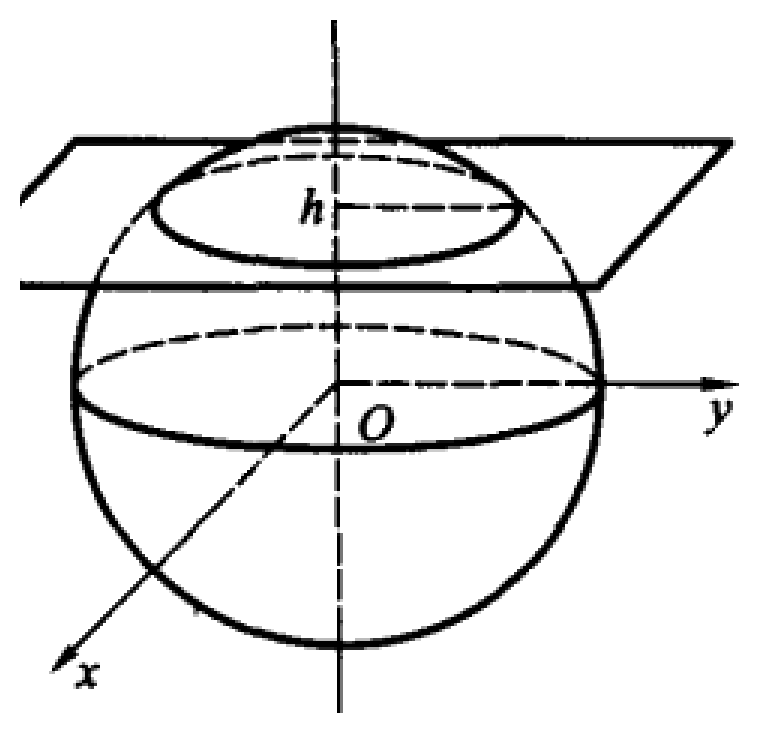
\includegraphics[width=0.42\textwidth]{work/figures/fig21-3}\caption{\relax}\label{fig:21-3}
\end{figure}

\begin{proof}[解]
曲面 $S$ 在 $Oxy$ 面上的投影区域 $D$ 为 $x^{2}+y^{2}\leqslant a^{2}-h^{2}$，而
\[
\sqrt{1+z_{x}^{2}(x,y)+z_{y}^{2}(x,y)}=\frac{a}{\sqrt{a^{2}-x^{2}-y^{2}}}.
\]
因此
\[
\begin{aligned}
\iint_{S}\frac{\mathrm{d}S}{z}&=\iint_{D}\frac{a}{a^{2}-x^{2}-y^{2}}\,\mathrm{d}x\mathrm{d}y\\
&=\int_{0}^{2\pi}\mathrm{d}\theta\int_{0}^{\sqrt{a^{2}-h^{2}}}\frac{a}{a^{2}-r^{2}}r\,\mathrm{d}r\\
&=\pi a\ln\left|a^{2}-r^{2}\right|\bigg|_{\sqrt{a^{2}-h^{2}}}^{0}\\
&=2a\pi\ln\frac{a}{h}.
\end{aligned}
\]
\end{proof}

\begin{example}\label{ex:21-2-2}
计算 $\displaystyle\iint_{S}(x+y+z)\,\mathrm{d}S$，其中 $S$ 是球面 $x^{2}+y^{2}+z^{2}=a^{2}$，$z\geqslant0$．
\end{example}

\begin{proof}[解]
本题用 $S$ 的参数方程更简便些，利用球坐标易写出 $S$ 的参数方程为
\[
\begin{cases}
x=a\cos\theta\sin\varphi,\\
y=a\sin\theta\sin\varphi,\\
z=a\cos\varphi,
\end{cases}
\quad 0\leqslant\theta\leqslant2\pi,\quad 0\leqslant\varphi\leqslant\frac{\pi}{2}.
\]
计算
\[
\begin{aligned}
\begin{pmatrix}x_{\theta}&y_{\theta}&z_{\theta}\\ x_{\varphi}&y_{\varphi}&z_{\varphi}\end{pmatrix}
&=\begin{pmatrix}-a\sin\theta\sin\varphi&a\cos\theta\sin\varphi&0\\ a\cos\theta\cos\varphi&a\sin\theta\cos\varphi&-a\sin\varphi\end{pmatrix},\\
E&=a^{2}\sin^{2}\varphi,\quad G=a^{2},\quad F=0.
\end{aligned}
\]
因此
\[
\begin{aligned}
&\iint_{S}(x+y+z)\,\mathrm{d}S\\
={}&\iint_{D}a(\cos\theta\sin\varphi+\sin\theta\sin\varphi+\cos\varphi)\sqrt{a^{4}\sin^{2}\varphi}\,\mathrm{d}\theta\mathrm{d}\varphi\\
={}&a^{3}\int_{0}^{\frac{\pi}{2}}\sin\varphi\,\mathrm{d}\varphi\int_{0}^{2\pi}(\cos\theta\sin\varphi+\sin\theta\sin\varphi+\cos\varphi)\,\mathrm{d}\theta\\
={}&2\pi a^{3}\int_{0}^{\frac{\pi}{2}}\sin\varphi\cos\varphi\,\mathrm{d}\varphi=\pi a^{3}.
\end{aligned}
\]
\end{proof}

读者不难发现此例中 $\displaystyle\iint_{S}x\,\mathrm{d}S=\iint_{S}y\,\mathrm{d}S=0$．$\iint_{S}x\,\mathrm{d}S=0$ 是因为曲面 $S$ 关于 $Oyz$ 平面对称，而被积函数是 $x$ 的奇函数．同理知 $\displaystyle\iint_{S}y\,\mathrm{d}S=0$．

\begin{example}\label{ex:21-2-3}
求均匀球壳对不在该球壳上的一单位质点 $M$ 的引力．设球壳的密度 $\rho=1$．
\end{example}

\begin{proof}[解]
为计算方便，选择质点位于 $z$ 轴上 $(0,0,h)$ 处 $(h>0)$，球壳的球心在原点，半径为 $R(R\neq h)$．

由对称性知引力 $\bm{F}$ 在 $x$ 轴和 $y$ 轴上的投影为零，故只要求 $\bm{F}$ 在 $z$ 轴上的投影 $F_{z}$．

任取面积微元 $\mathrm{d}S$，它对 $M$ 的引力为
\[
\mathrm{d}\bm{F}=\frac{k_{\rho}\,\mathrm{d}S}{r^{2}}\bm{r}_{0},
\]
其中 $r=\sqrt{x^{2}+y^{2}+(z-h)^{2}}$，$\bm{r}_{0}=\dfrac{1}{r}(x,y,z-h)$，$\rho=1$．因此 $\mathrm{d}\bm{F}$ 在 $z$ 轴上的投影为
\[
\mathrm{d}F_{z}=\frac{k(z-h)}{r^{3}}\,\mathrm{d}S.
\]
故
\[
F_{z}=\iint_{S}\frac{k(z-h)}{r^{3}}\,\mathrm{d}S.
\]
用球面的参数方程
\[
\begin{cases}
x=R\cos\theta\sin\varphi,\\
y=R\sin\theta\sin\varphi,\\
z=R\cos\varphi,
\end{cases}
\quad 0\leqslant\theta\leqslant2\pi,\qquad 0\leqslant\varphi\leqslant\pi,
\]
则
\[
\begin{aligned}
\mathrm{d}S&=\sqrt{EG-F^{2}}\,\mathrm{d}\theta\mathrm{d}\varphi=R^{2}\sin\varphi\,\mathrm{d}\theta\mathrm{d}\varphi,\\
r&=\sqrt{R^{2}+h^{2}-2Rh\cos\varphi}.
\end{aligned}
\]
从而
\[
\begin{aligned}
F_{z}&=\int_{0}^{2\pi}\mathrm{d}\theta\int_{0}^{\pi}\frac{k(R\cos\varphi-h)}{(R^{2}+h^{2}-2Rh\cos\varphi)^{\frac{3}{2}}}R^{2}\sin\varphi\,\mathrm{d}\varphi\\
&=2\pi kR^{2}\int_{0}^{\pi}\frac{R\cos\varphi-h}{(R^{2}+h^{2}-2Rh\cos\varphi)^{\frac{3}{2}}}\sin\varphi\,\mathrm{d}\varphi\\
&=\frac{\pi kR^{2}}{h}\int_{0}^{\pi}\frac{(R^{2}+h^{2}-2Rh\cos\varphi)+2h^{2}-h^{2}-R^{2}}{(R^{2}+h^{2}-2Rh\cos\varphi)^{\frac{3}{2}}}\,\mathrm{d}\cos\varphi\\
&=\frac{\pi kR^{2}}{h}\left[\int_{0}^{\pi}\frac{\mathrm{d}\cos\varphi}{(R^{2}+h^{2}-2Rh\cos\varphi)^{\frac{1}{2}}}+\int_{0}^{\pi}\frac{(h^{2}-R^{2})\,\mathrm{d}\cos\varphi}{(R^{2}+h^{2}-2Rh\cos\varphi)^{\frac{3}{2}}}\right]\\
&=\frac{\pi kR^{2}}{h}\left[\frac{1}{Rh}\sqrt{R^{2}+h^{2}-2Rh\cos\varphi}\,\Bigg|_{\pi}^{0}-\frac{h^{2}-R^{2}}{Rh}\frac{1}{\sqrt{R^{2}+h^{2}-2Rh\cos\varphi}}\,\Bigg|_{\pi}^{0}\right]\\
&=\frac{\pi kR}{h^{2}}\left[|R-h|-(R+h)-(h^{2}-R^{2})\left(\frac{1}{|R-h|}-\frac{1}{R+h}\right)\right]\\
&=\begin{cases}
-\dfrac{4\pi kR^{2}}{h^{2}},&h>R,\\[4pt]
0,&h<R.
\end{cases}
\end{aligned}
\]
\end{proof}

\begin{figure}[htbp]
\centering
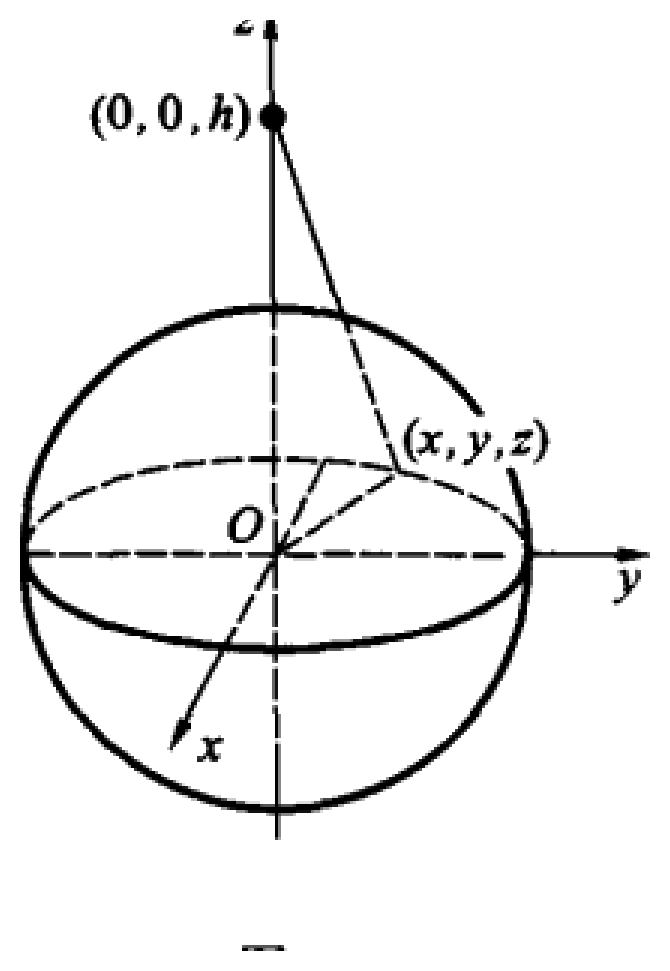
\includegraphics[width=0.45\textwidth]{work/figures/fig21-4}\caption{\relax}\label{fig:21-4}
\end{figure}

这个结果表明：均匀球壳内的任一点所受球壳的引力处于平衡状态，而均匀球壳外的点所受球壳的引力等于把球壳的全部质量集中到球心时对该点的引力．

\begin{xiti}
\item 对照重积分的基本性质写出第一型曲线积分和第一型曲面积分的类似性质．
\item 计算下列第一型曲线积分：
\begin{ziti}
\item $\displaystyle\int_{L}(x^{2}+y^{2})\,\mathrm{d}s$，其中 $L$ 是以 $(0,0)$，$(2,0)$，$(0,1)$ 为顶点的三角形；
\item $\displaystyle\int_{L}\sqrt{x^{2}+y^{2}}\,\mathrm{d}s$，其中 $L$ 是圆周 $x^{2}+y^{2}=ax$；
\item $\displaystyle\int_{L}xyz\,\mathrm{d}s$，其中 $L$ 为螺线 $x=a\cos t$，$y=a\sin t$，$z=bt$ $(0<a<b)$，$0\leqslant t\leqslant2\pi$；
\item $\displaystyle\int_{L}(x^{2}+y^{2}+z^{2})\,\mathrm{d}s$，其中 $L$ 与（3）相同；
\item $\displaystyle\int_{L}\left(x^{\frac{4}{3}}+y^{\frac{4}{3}}\right)\mathrm{d}s$，其中 $L$ 为内摆线 $x^{\frac{2}{3}}+y^{\frac{2}{3}}=a^{\frac{2}{3}}$；
\item $\displaystyle\int_{L}y^{2}\,\mathrm{d}s$，其中 $L$ 为摆线的一拱 $x=a(t-\sin t)$，$y=a(1-\cos t)$，$0\leqslant t\leqslant2\pi$；
\item $\displaystyle\int_{L}xy\,\mathrm{d}s$，其中 $L$ 为球面 $x^{2}+y^{2}+z^{2}=a^{2}$ 与平面 $x+y+z=0$ 的交线；
\item $\displaystyle\int_{L}(xy+yz+zx)\,\mathrm{d}s$，其中 $L$ 同（7）；
\item $\displaystyle\int_{L}xyz\,\mathrm{d}s$，其中 $L$ 是曲线 $x=t$，$y=\dfrac{2}{3}\sqrt{2t^{3}}$，$z=\dfrac{1}{2}t^{2}$ $(0\leqslant t\leqslant1)$；
\item $\displaystyle\int_{L}\sqrt{2y^{2}+z^{2}}\,\mathrm{d}s$，其中 $L$ 是 $x^{2}+y^{2}+z^{2}=a^{2}$ 与 $x=y$ 相交的圆周．
\end{ziti}
\item 计算下列第一型曲面积分：
\begin{ziti}
\item $\displaystyle\iint_{S}(x^{2}+y^{2})\,\mathrm{d}S$，其中 $S$ 是立体 $\sqrt{x^{2}+y^{2}}\leqslant z\leqslant1$ 的边界曲面；
\item $\displaystyle\iint_{S}\frac{\mathrm{d}S}{x^{2}+y^{2}}$，其中 $S$ 为柱面 $x^{2}+y^{2}=R^{2}$ 被平面 $z=0$ 和 $z=H$ 所截取的部分；
\item $\displaystyle\iint_{S}\left|x^{3}y^{2}z\right|\,\mathrm{d}S$，其中 $S$ 是曲面 $z=x^{2}+y^{2}$ 被平面 $z=1$ 割下的部分；
\item $\displaystyle\iint_{S}z^{2}\,\mathrm{d}S$，其中 $S$ 为螺旋面的一部分：
\[
x=u\cos v,\quad y=u\sin v,\quad z=v\quad\left(0\leqslant u\leqslant a,\,0\leqslant v\leqslant2\pi\right)
\]；
\item $\displaystyle\iint_{S}(x^{2}+y^{2})\,\mathrm{d}S$，$S$ 是球面 $x^{2}+y^{2}+z^{2}=R^{2}$．
\end{ziti}
\item 设曲线 $L$ 的方程为
\[
x=\mathrm{e}^{t}\cos t,\quad y=\mathrm{e}^{t}\sin t,\quad z=\mathrm{e}^{t}\quad\left(0\leqslant t\leqslant t_{0}\right),
\]
它在每一点的密度与该点的矢径平方成反比，且在点 $(1,0,1)$ 处为 $1$，求它的质量．
\item 设有一质量分布不均匀的半圆弧 $x=r\cos\theta$，$y=r\sin\theta$ $(0\leqslant\theta\leqslant\pi)$，其线密度 $\rho=a\theta$（$a$ 为常数），求它对原点 $(0,0)$ 处质量为 $m$ 的质点的引力．
\item 求螺线的一支 $L$：$x=a\cos t$，$y=a\sin t$，$z=\dfrac{h}{2\pi}t$ $(0\leqslant t\leqslant2\pi)$ 对 $x$ 轴的转动惯量 $I=\displaystyle\int_{L}(y^{2}+z^{2})\,\mathrm{d}s$．设此螺线的线密度是均匀的．
\item 求抛物面壳 $z=\dfrac{1}{2}(x^{2}+y^{2})$，$0\leqslant z\leqslant1$ 的质量．设此壳的密度 $\rho=z$．
\item 计算球面三角形 $x^{2}+y^{2}+z^{2}=a^{2}$，$x>0$，$y>0$，$z>0$ 的围线的重心坐标．设线密度 $\rho=1$．
\item 求均匀球壳 $x^{2}+y^{2}+z^{2}=a^{2}$ $(z\geqslant0)$ 对 $z$ 轴的转动惯量．
\item 求均匀球面 $z=\sqrt{a^{2}-x^{2}-y^{2}}$ $(x\geqslant0,\,y\geqslant0,\,x+y\leqslant a)$ 的重心坐标．
\item 若曲线以极坐标给出：$\rho=\rho(\theta)$ $(\theta_{1}\leqslant\theta\leqslant\theta_{2})$，试给出计算 $\displaystyle\int_{L}f(x,y)\,\mathrm{d}s$ 的公式，并用此公式计算下列曲线积分：
\begin{ziti}
\item $\displaystyle\int_{L}e^{\sqrt{x^{2}+y^{2}}}\,\mathrm{d}s$，其中 $L$ 是曲线 $\rho=a$ $\left(0\leqslant\theta\leqslant\dfrac{\pi}{4}\right)$；
\item $\displaystyle\int_{L}x\,\mathrm{d}s$，其中 $L$ 是对数螺线 $\rho=a\mathrm{e}^{k\theta}$ $(k>0)$ 在圆 $r=a$ 内的部分．
\end{ziti}
\item 求密度 $\rho=\rho_{0}$ 的截圆锥面 $x=r\cos\varphi$，$y=r\sin\varphi$，$z=r$ $(0\leqslant\varphi\leqslant2\pi)$，$0<b\leqslant r\leqslant a$ 对位于曲面顶点 $(0,0,0)$ 的单位质点的引力．当 $b\to0$ 时，结果如何？
\item 计算 $F(t)=\iint_{S}f(x,y,z)\,\mathrm{d}S$，其中 $S$ 是一平面 $x+y+z=t$，而
\[
f(x,y,z)=\begin{cases}
1-x^{2}-y^{2}-z^{2},&\text{当}\ x^{2}+y^{2}+z^{2}\leqslant1,\\
0,&\text{当}\ x^{2}+y^{2}+z^{2}>1.
\end{cases}
\]
\end{xiti}

\section{第二型曲线积分与曲面积分}

第一型曲线积分和曲面积分，其曲线和曲面都是无方向的，本质上与二重积分和三重积分是同类型的积分．这一节要介绍的第二型曲线积分和曲面积分，其曲线和曲面是有方向的．其实这种类型的积分我们并不陌生，定积分 $\displaystyle\int_{a}^{b}f(x)\,\mathrm{d}x$ 的区间就是有方向的：从 $a$ 到 $b$．如果反方向，便会差一个负号
\[
\int_{b}^{a}f(x)\,\mathrm{d}x=-\int_{a}^{b}f(x)\,\mathrm{d}x.
\]
曲线有方向，比较容易理解．什么叫曲面的方向？下面我们从物理背景开始，引进第二型的曲线与曲面积分．

\subsection{变力作功与第二型曲线积分}

设一质点受变力 $\bm{F}(x,y,z)$ 的作用沿空间光滑曲线段 $L$ 从点 $A$ 运动到点 $B$，变力 $\bm{F}(x,y,z)$ 不仅大小随点的变化而变化，而且方向也随点的变化而变化．这时力 $\bm{F}(x,y,z)$ 所作的功应如何计算呢？

从 $A$ 向 $B$ 给曲线弧 $L$ 一个分法：
\[
A=M_{0},M_{1},M_{2},\cdots,M_{n}=B,
\]
其中 $M_{i}=(x_{i},y_{i},z_{i})$．记 $\widehat{M_{i-1}M_{i}}$ 的弧长为 $\Delta s_{i}$，任取 $(\xi_{i},\eta_{i},\zeta_{i})\in\widehat{M_{i-1}M_{i}}$．当 $\lambda=\max\limits_{1\leqslant i\leqslant n}\{\Delta s_{i}\}$ 很小时，每个小弧段 $\widehat{M_{i-1}M_{i}}$ 上的力近似于常力 $\bm{F}(\xi_{i},\eta_{i},\zeta_{i})$，而力 $\bm{F}(x,y,z)$ 使质点沿 $\widehat{M_{i-1}M_{i}}$ 从 $M_{i-1}$ 运动到 $M_{i}$ 所作的功 $W_{i}$ 有下面的近似表达式
\[
W_{i}\approx\bm{F}(\xi_{i},\eta_{i},\zeta_{i})\cdot\overrightarrow{M_{i-1}M_{i}}.
\]
因此 $\bm{F}(x,y,z)$ 使质点从 $A$ 运动到 $B$ 所作的功
\[
W\approx\sum_{i=1}^{n}\bm{F}(\xi_{i},\eta_{i},\zeta_{i})\cdot\overrightarrow{M_{i-1}M_{i}}.
\]
$\lambda$ 越小近似程度越好．故当 $\lambda\to0$ 时，上式右端和的极限就是 $\bm{F}(x,y,z)$ 使质点从 $A$ 运动到 $B$ 所作的功．

\begin{figure}[htbp]
\centering
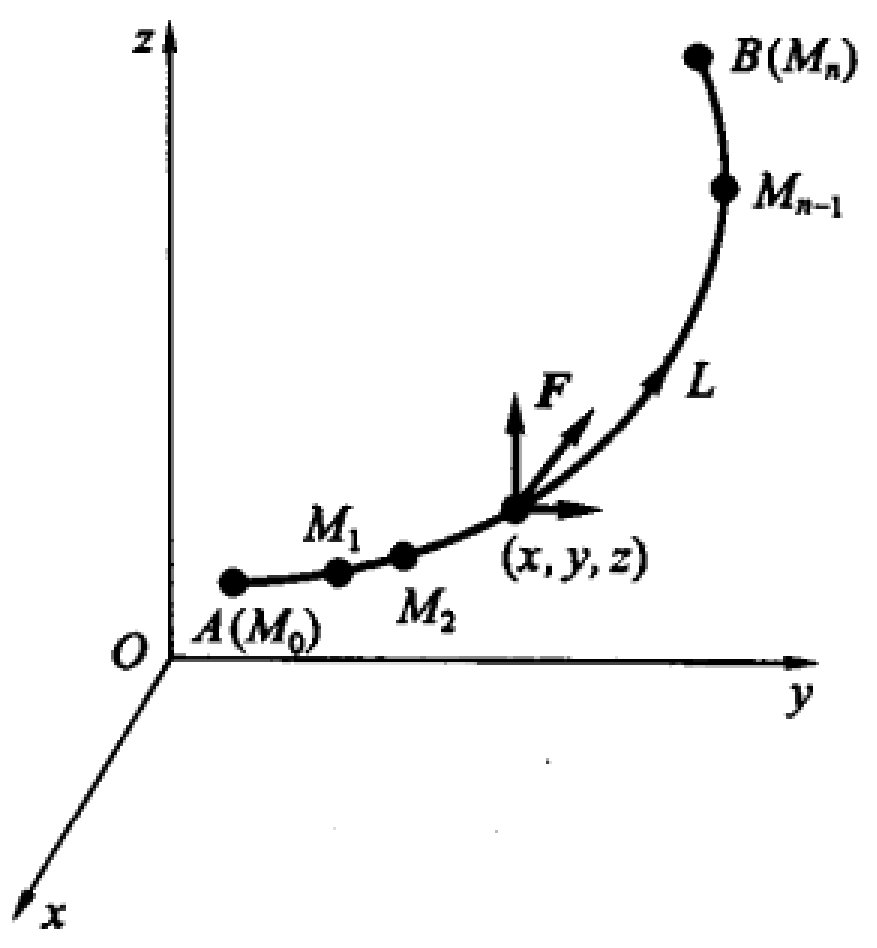
\includegraphics[width=0.4\textwidth]{work/figures/fig21-5}\caption{\relax}\label{fig:21-5}
\end{figure}

因为
\[
\begin{aligned}
\overrightarrow{M_{i-1}M_{i}}&=(x_{i}-x_{i-1},y_{i}-y_{i-1},z_{i}-z_{i-1})\\
&=(\Delta x_{i},\Delta y_{i},\Delta z_{i}),
\end{aligned}
\]
注意这时 $\Delta x_{i},\Delta y_{i},\Delta z_{i}$ 是可正可负的，大小与符号由向量 $\overrightarrow{M_{i-1}M_{i}}$ 决定．又若
\[
\bm{F}(x,y,z)=\left(P(x,y,z),Q(x,y,z),R(x,y,z)\right)
\]
则有
\[
\begin{aligned}
W&=\lim_{\lambda\to0}\sum_{i=1}^{n}\bm{F}(\xi_{i},\eta_{i},\zeta_{i})\cdot\overrightarrow{M_{i-1}M_{i}}\\
&=\lim_{\lambda\to0}\left\{\sum_{i=1}^{n}P(\xi_{i},\eta_{i},\zeta_{i})\Delta x_{i}+Q(\xi_{i},\eta_{i},\zeta_{i})\Delta y_{i}+R(\xi_{i},\eta_{i},\zeta_{i})\Delta z_{i}\right\}.
\end{aligned}
\]
抽去其中的物理背景，这样一种和的极限就引导到第二型曲线积分．

\begin{definition}\label{def:21-3}
设函数 $f(x,y,z)$ 定义在空间光滑曲线弧 $L$ 上，$L$ 的两端点为 $A$，$B$．从 $A$ 向 $B$ 给 $\widehat{AB}$ 一个分法：$A=M_{0},M_{1},\cdots,M_{n}=B$，其中 $M_{i}=(x_{i},y_{i},z_{i})$，记 $\widehat{M_{i-1}M_{i}}$ 的弧长为 $\Delta s_{i}$，$\Delta x_{i}=x_{i}-x_{i-1}$，任取 $(\xi_{i},\eta_{i},\zeta_{i})\in\widehat{M_{i-1}M_{i}}$，作和式
\[
\sigma=\sum_{i=1}^{n}f(\xi_{i},\eta_{i},\zeta_{i})\Delta x_{i}.
\]
若当 $\lambda=\max\limits_{1\leqslant i\leqslant n}\{\Delta s_{i}\}\to0$ 时，$\sigma$ 的极限存在，则称该极限为函数 $f$ 沿有向曲线 $L$ 对 $x$ 的\emph{第二型曲线积分}，记为
\[
\int_{L}f(x,y,z)\,\mathrm{d}x,
\]
或
\[
\int_{\widehat{AB}}f(x,y,z)\,\mathrm{d}x.
\]
如果在上述求和时，分别用 $\Delta y_{i}=y_{i}-y_{i-1}$ 或 $\Delta z_{i}=z_{i}-z_{i-1}$ 代替 $\Delta x_{i}$，便得到 $f$ 沿 $L$ 对 $y$ 或对 $z$ 的第二型曲线积分：
\[
\int_{L}f(x,y,z)\,\mathrm{d}y
\]
或
\[
\int_{L}f(x,y,z)\,\mathrm{d}z.
\]
\end{definition}

如果有向量函数 $\bm{F}(x,y,z)=\left(P(x,y,z),Q(x,y,z),R(x,y,z)\right)$，则根据定义~\ref{def:21-3} 有
\[
\begin{aligned}
&\int_{L}P(x,y,z)\,\mathrm{d}x+\int_{L}Q(x,y,z)\,\mathrm{d}y+\int_{L}R(x,y,z)\,\mathrm{d}z\\
={}&\lim_{\lambda\to0}\sum_{i=1}^{n}\left[P(\xi_{i},\eta_{i},\zeta_{i})\Delta x_{i}+Q(\xi_{i},\eta_{i},\zeta_{i})\Delta y_{i}+R(\xi_{i},\eta_{i},\zeta_{i})\Delta z_{i}\right],
\end{aligned}
\]
其中 $\Delta x_{i}$，$\Delta y_{i}$，$\Delta z_{i}$ 分别是向量 $\overrightarrow{M_{i-1}M_{i}}$ 在 $x$，$y$，$z$ 轴上的有向投影．若记
\[
\mathrm{d}\bm{s}=\left\{\mathrm{d}x,\mathrm{d}y,\mathrm{d}z\right\},
\]
则
\[
\begin{aligned}
&\int_{L}P(x,y,z)\,\mathrm{d}x+Q(x,y,z)\,\mathrm{d}y+R(x,y,z)\,\mathrm{d}z\\
={}&\int_{L}\bm{F}(x,y,z)\cdot\mathrm{d}\bm{s}.
\end{aligned}
\]
因此上述积分也称为向量函数 $\bm{F}(x,y,z)$ 沿有向曲线 $L$ 的积分．$\mathrm{d}\bm{s}$ 的方向就是曲线 $L$ 的切线方向，其指向与 $L$ 的方向一致．

第二型曲线积分中曲线是有方向的，这是与第一型曲线积分的根本区别所在．如果对 $L$ 的积分改为由 $B$ 到 $A$，则在上述定义中，变成了用 $\overrightarrow{M_{i}M_{i-1}}$ 的投影来代替原来的 $\overrightarrow{M_{i-1}M_{i}}$ 的投影，显然和式差了一个负号．因此对同一曲线有
\[
\int_{\widehat{AB}}P\,\mathrm{d}x+Q\,\mathrm{d}y+R\,\mathrm{d}z=-\int_{\widehat{BA}}P\,\mathrm{d}x+Q\,\mathrm{d}y+R\,\mathrm{d}z.
\]
它们恰好相差一个负号．而对第一型曲线积分来说，从 $A$ 到 $B$ 的积分与从 $B$ 到 $A$ 的积分是相等的，即
\[
\int_{\widehat{AB}}f(x,y,z)\,\mathrm{d}s=\int_{\widehat{BA}}f(x,y,z)\,\mathrm{d}s.
\]
对于闭曲线 $L$，我们常记为
\[
\oint_{L}P\,\mathrm{d}x+Q\,\mathrm{d}y+R\,\mathrm{d}z.
\]
这时积分与起点的选择无关，只与曲线 $L$ 的方向有关．

下面的定理告诉我们，连续函数沿光滑线段的第二型曲线积分总存在，并且可以化为定积分来计算．

\begin{theorem}\label{thm:21-3}
设 $f(x,y,z)$ 是定义在光滑曲线段
\[
\widehat{AB}:x=x(t),\ y=y(t),\ z=z(t),\quad\alpha\leqslant t\leqslant\beta
\]
上的连续函数，$t=\alpha$ 时对应于 $A$ 点，$t=\beta$ 时对应于 $B$ 点，且 $\widehat{AB}$ 自身不相交，则 $f$ 沿 $\widehat{AB}$ 的第二型曲线积分 $\displaystyle\int_{\widehat{AB}}f(x,y,z)\,\mathrm{d}x$ 存在，且有
\[
\int_{\widehat{AB}}f(x,y,z)\,\mathrm{d}x=\int_{\alpha}^{\beta}f(x(t),y(t),z(t))x^{\prime}(t)\,\mathrm{d}t.
\]
\end{theorem}

\begin{proof}
从 $A$ 向 $B$ 任给 $\widehat{AB}$ 一个分法 $A=M_{0},M_{1},\cdots,M_{n}=B$，$M_{i}=(x_{i},y_{i},z_{i})$ $(i=0,1,\cdots,n)$，则相应地得到 $[\alpha,\beta]$ 的一个分法：
\[
\alpha=t_{0}<t_{1}<\cdots<t_{n}=\beta,
\]
使得 $M_{i}=(x(t_{i}),y(t_{i}),z(t_{i}))$ $(i=1,2,\cdots,n)$．由于 $\widehat{AB}$ 自身不相交，故上述 $M_{i}$ 与 $t_{i}$ 是一一对应的．任取 $(\xi_{i},\eta_{i},\zeta_{i})\in\widehat{M_{i-1}M_{i}}$，存在 $\tau_{i}\in[t_{i-1},t_{i}]$，使
\[
(\xi_{i},\eta_{i},\zeta_{i})=(x(\tau_{i}),y(\tau_{i}),z(\tau_{i})).
\]
因此
\[
\begin{aligned}
\sigma&=\sum_{i=1}^{n}f(\xi_{i},\eta_{i},\zeta_{i})\Delta x_{i}\\
&=\sum_{i=1}^{n}f(x(\tau_{i}),y(\tau_{i}),z(\tau_{i}))\left(x(t_{i})-x(t_{i-1})\right).
\end{aligned}
\]
由于 $\widehat{AB}$ 是光滑曲线，$x(t)$ 在 $[\alpha,\beta]$ 有连续导数，由拉格朗日中值定理，存在 $\tau_{i}^{*}\in[t_{i-1},t_{i}]$，使
\[
x(t_{i})-x(t_{i-1})=x^{\prime}(\tau_{i}^{*})(t_{i}-t_{i-1})=x^{\prime}(\tau_{i}^{*})\Delta t_{i}.
\]
因此
\[
\sigma=\sum_{i=1}^{n}f(x(\tau_{i}),y(\tau_{i}),z(\tau_{i}))x^{\prime}(\tau_{i}^{*})\Delta t_{i}.
\]
记 $\lambda=\max\limits_{1\leqslant i\leqslant n}\{\Delta s_{i}\}$，$\lambda'=\max\limits_{1\leqslant i\leqslant n}\{\Delta t_{i}\}$，因为 $\widehat{AB}$ 是光滑曲线，故当 $\lambda\to0$ 时有 $\lambda'\to0$．又由于 $f(x(t),y(t),z(t))$，$x'(t)$ 都在 $[\alpha,\beta]$ 连续，虽然 $\tau_{i}$，$\tau_{i}^{*}\in[t_{i-1},t_{i}]$ 不一定相同，但像我们以前证明过多次的一样，$\sigma$ 的极限是存在的，且
\[
\begin{aligned}
&\lim_{\lambda\to0}\sum_{i=1}^{n}f(x(\tau_{i}),y(\tau_{i}),z(\tau_{i}))x^{\prime}(\tau_{i}^{*})\Delta t_{i}\\
={}&\int_{\alpha}^{\beta}f(x(t),y(t),z(t))x^{\prime}(t)\,\mathrm{d}t.
\end{aligned}
\]
而根据定义，$\sigma$ 的极限是曲线积分 $\displaystyle\int_{\widehat{AB}}f(x,y,z)\,\mathrm{d}x$，这就完成了定理~\ref{thm:21-3} 的证明．
\end{proof}

类似地可以证明在定理~\ref{thm:21-3} 的条件下有
\[
\int_{\widehat{AB}}f(x,y,z)\,\mathrm{d}y=\int_{\alpha}^{\beta}f(x(t),y(t),z(t))y^{\prime}(t)\,\mathrm{d}t.
\]
\[
\int_{\widehat{AB}}f(x,y,z)\,\mathrm{d}z=\int_{\alpha}^{\beta}f(x(t),y(t),z(t))z^{\prime}(t)\,\mathrm{d}t.
\]
要特别强调的是公式右端定积分的下限总是对应有向曲线段的起点，上限总是对应有向曲线段的终点．

如果曲线 $L$ 是分段光滑的有向曲线，那么 $L$ 是有限条光滑曲线段连结而成且上一段的终点是下一段的起点，这时公式仍然成立．事实上只要逐段地应用上述公式再对积分值求和即可．

\begin{example}\label{ex:21-3-1}
求 $\displaystyle\int_{\widehat{AB}}(x^{2}+y^{2})\,\mathrm{d}x+4xy\,\mathrm{d}y$，其中
\begin{ziti}
\item $\widehat{AB}$ 是上半圆周 $x^{2}+y^{2}=ax$ $(y\geqslant0)$，
\item $\widehat{AB}$ 是直线段 $y=0$ $(0\leqslant x\leqslant a)$，
\end{ziti}
方向如图~\ref{fig:21-6} 所示．
\end{example}

\begin{figure}[htbp]
\centering
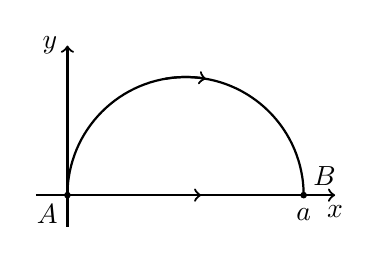
\begin{tikzpicture}[scale=1]
\draw[->,thick] (-0.4,0) -- (3.4,0) node[below] {$x$};
\draw[->,thick] (0,-0.4) -- (0,1.9) node[left] {$y$};
\draw[thick] (0,0) arc (180:0:1.5);
\draw[thick,->] ({1.5+1.5*cos(100)},{1.5*sin(100)}) arc (100:80:1.5);
\fill (0,0) circle (1.2pt) node[below left] {$A$};
\fill (3,0) circle (1.2pt) node[above right] {$B$};
\node[below] at (3,-0.05) {$a$};
\draw[thick,->] (1.3,0) -- (1.7,0);
\end{tikzpicture}\caption{\relax}\label{fig:21-6}
\end{figure}

\begin{proof}[解]
（1）取 $\widehat{AB}$ 的参数方程为
\[
\begin{cases}
x=x,\\
y=\sqrt{ax-x^{2}},
\end{cases}
\quad 0\leqslant x\leqslant a.
\]
\[
\begin{aligned}
&\int_{\widehat{AB}}\left(x^{2}+y^{2}\right)\mathrm{d}x+4xy\,\mathrm{d}y\\
={}&\int_{0}^{a}\left[x^{2}+\left(ax-x^{2}\right)+4x\sqrt{ax-x^{2}}\,\frac{a-2x}{2\sqrt{ax-x^{2}}}\right]\mathrm{d}x\\
={}&\int_{0}^{a}(3ax-4x^{2})\,\mathrm{d}x=\frac{a^{3}}{6}.
\end{aligned}
\]
我们也可以取 $\widehat{AB}$ 的参数方程为
\[
\begin{cases}
x=\dfrac{a}{2}+\dfrac{a}{2}\cos\theta,\\
y=\dfrac{a}{2}\sin\theta,
\end{cases}
\quad 0\leqslant\theta\leqslant\pi.
\]
注意 $\theta=\pi$ 时对应于 $A$ 点，$\theta=0$ 时对应于 $B$ 点，因此
\[
\begin{aligned}
&\int_{\widehat{AB}}\left(x^{2}+y^{2}\right)\mathrm{d}x+4xy\,\mathrm{d}y\\
={}&\int_{\pi}^{0}\left\{\left[\left(\frac{a}{2}+\frac{a}{2}\cos\theta\right)^{2}+\left(\frac{a}{2}\sin\theta\right)^{2}\right]\left(-\frac{a}{2}\sin\theta\right)+\right.\\
&\left.\phantom{\int_{\pi}^{0}}4\left(\frac{a}{2}+\frac{a}{2}\cos\theta\right)\frac{a}{2}\sin\theta\,\frac{a}{2}\cos\theta\right\}\mathrm{d}\theta\\
={}&\int_{\pi}^{0}\left(\frac{a}{2}\right)^{3}\left[-(2+2\cos\theta)\sin\theta+4(1+\cos\theta)\sin\theta\cos\theta\right]\mathrm{d}\theta\\
={}&\left(\frac{a}{2}\right)^{3}\int_{\pi}^{0}\left(-2\sin\theta+4\cos^{2}\theta\sin\theta\right)\mathrm{d}\theta\\
={}&\left(\frac{a}{2}\right)^{3}\left[2\cos\theta-\frac{4}{3}\cos^{3}\theta\right]\Bigg|_{\pi}^{0}=\frac{a^{3}}{6},
\end{aligned}
\]
其中第三个等式用到了正交性
\[
\int_{0}^{\pi}\sin\theta\cos\theta\,\mathrm{d}\theta=0.
\]
（2）因为 $y=0$，$\mathrm{d}y=0$，故
\[
\int_{\widehat{AB}}\left(x^{2}+y^{2}\right)\mathrm{d}x+4xy\,\mathrm{d}y=\int_{0}^{a}x^{2}\,\mathrm{d}x=\frac{x^{3}}{3}\bigg|_{0}^{a}=\frac{a^{3}}{3}.
\]
\end{proof}

从此例可见尽管两曲线的起点和终点相同．但由于路径不同，积分值可能不同．进一步（1）、（2）中的两曲线段构成封闭曲线 $L$，则沿 $L$ 的逆时针方向有
\[
\int_{L}\left(x^{2}+y^{2}\right)\mathrm{d}x+4xy\,\mathrm{d}y=-\frac{a^{3}}{6}+\frac{a^{3}}{3}=\frac{a^{3}}{6}.
\]

\begin{example}\label{ex:21-3-2}
求在力 $\bm{F}=(y,-x,x+y+z)$ 的作用下，质点由 $A$ 到 $B$ 所作的功（图~\ref{fig:21-7}）：
\begin{ziti}
\item $\widehat{AB}$ 是螺旋线
\[
L_{1}:x=a\cos t,\quad y=a\sin t,\quad z=bt,\quad 0\leqslant t\leqslant2\pi;
\]
\item $\widehat{AB}$ 是直线段
\[
L_{2}:\ x=a,\ y=0,\ z=t,\ 0\leqslant t\leqslant2\pi b.
\]
\end{ziti}
\end{example}

\begin{figure}[htbp]
\centering
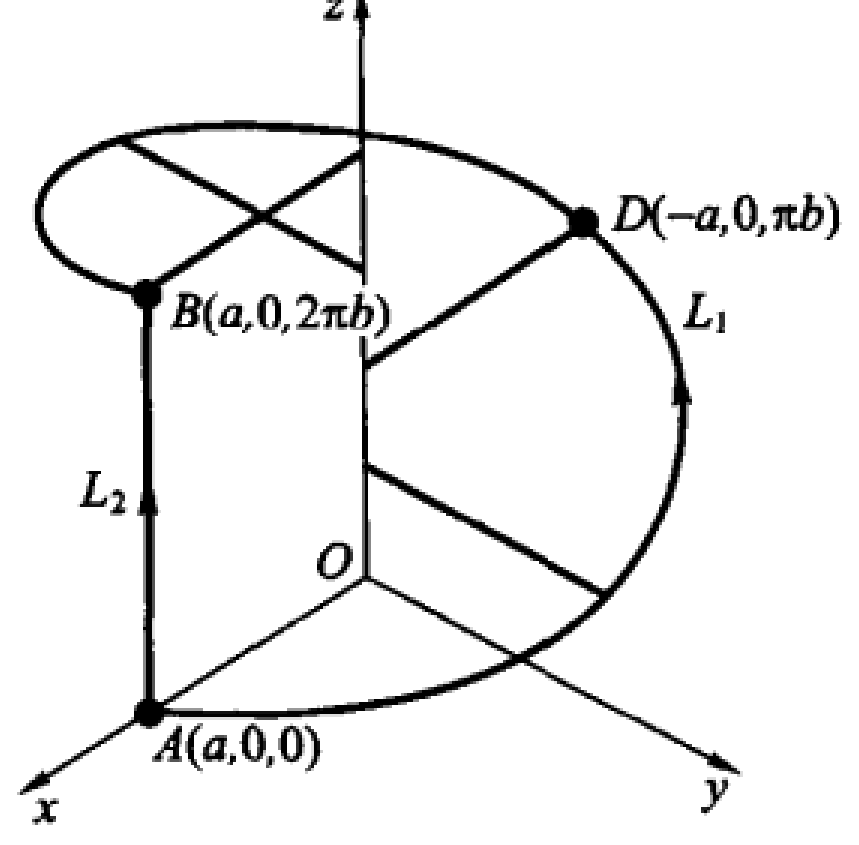
\includegraphics[width=0.45\textwidth]{work/figures/fig21-7}\caption{\relax}\label{fig:21-7}
\end{figure}

\begin{proof}[解]
（1）
\[
\begin{aligned}
W&=\int_{L_{1}}\bm{F}\cdot\mathrm{d}\bm{s}\\
&=\int_{L_{1}}y\,\mathrm{d}x-x\,\mathrm{d}y+(x+y+z)\,\mathrm{d}z\\
&=\int_{0}^{2\pi}\left[-(a\sin t)^{2}-(a\cos t)^{2}+\right.\\
&\quad\left.\left(a\cos t+a\sin t+bt\right)b\right]\mathrm{d}t\\
&=\int_{0}^{2\pi}\left(-a^{2}+b^{2}t\right)\mathrm{d}t=2\pi(\pi b^{2}-a^{2}).
\end{aligned}
\]
（2）
\[
\begin{aligned}
W&=\int_{L_{2}}\bm{F}\cdot\mathrm{d}\bm{s}\\
&=\int_{L_{2}}y\,\mathrm{d}x-x\,\mathrm{d}y+(x+y+z)\,\mathrm{d}z\\
&=\int_{0}^{2\pi b}(a+t)\,\mathrm{d}t=2\pi b(a+\pi b).
\end{aligned}
\]
\end{proof}

我们曾经强调，从概念上说两型曲线积分是很不同的，但它们的计算都是化为定积分来完成，因此两者之间是有联系的．下面我们以定积分为桥梁，寻求两者之间的联系．

设光滑曲线段 $\widehat{AB}$ 的弧长为 $l$，$M$ 是 $\widehat{AB}$ 上的点．取弧长 $s=\widehat{AM}$ 为参数，得 $\widehat{AB}$ 的本性方程
\[
\begin{cases}
x=x(s),\\
y=y(s),\\
z=z(s),
\end{cases}
\quad 0\leqslant s\leqslant l.
\]
这时 $s$ 增加的方向就是 $\widehat{AB}$ 的方向．设 $P$，$Q$，$R$ 在 $\widehat{AB}$ 上连续，由第二型曲线积分的计算公式有
\[
\int_{\widehat{AB}}P(x,y,z)\,\mathrm{d}x=\int_{0}^{l}P(x(s),y(s),z(s))x^{\prime}(s)\,\mathrm{d}s,
\]
\[
\int_{\widehat{AB}}Q(x,y,z)\,\mathrm{d}y=\int_{0}^{l}Q(x(s),y(s),z(s))y^{\prime}(s)\,\mathrm{d}s,
\]
\[
\int_{\widehat{AB}}R(x,y,z)\,\mathrm{d}z=\int_{0}^{l}R(x(s),y(s),z(s))z^{\prime}(s)\,\mathrm{d}s.
\]
已知在 $M$ 点曲线的切向量为 $\bm{\tau}=(x^{\prime}(s),y^{\prime}(s),z^{\prime}(s))$，其方向与 $s$ 增加的方向一致，也就是 $\widehat{AB}$ 的方向．由于参数是弧长，而弧长
\[
s=\int_{0}^{s}\sqrt{x^{\prime2}(t)+y^{\prime2}(t)+z^{\prime2}(t)}\,\mathrm{d}t,
\]
因此
\[
\mathrm{d}s=\sqrt{x^{\prime2}(s)+y^{\prime2}(s)+z^{\prime2}(s)}\,\mathrm{d}s,
\]
即 $x^{\prime2}(s)+y^{\prime2}(s)+z^{\prime2}(s)=1$，这表明 $\bm{\tau}$ 是单位向量．用 $(\bm{\tau},x)$，$(\bm{\tau},y)$，$(\bm{\tau},z)$ 分别表示 $\bm{\tau}$ 与 $x$，$y$，$z$ 轴正向的夹角，就有
\[
\begin{aligned}
\bm{\tau}&=\left(x^{\prime}(s),y^{\prime}(s),z^{\prime}(s)\right)\\
&=\left(\cos(\bm{\tau},x),\cos(\bm{\tau},y),\cos(\bm{\tau},z)\right),
\end{aligned}
\]
故
\begin{align}
&\int_{\widehat{AB}}P\,\mathrm{d}x+Q\,\mathrm{d}y+R\,\mathrm{d}z\notag\\
={}&\int_{0}^{l}\left[Px^{\prime}(s)+Qy^{\prime}(s)+Rz^{\prime}(s)\right]\mathrm{d}s\tag{1}\label{eq:21-2-1}\\
={}&\int_{\widehat{AB}}\left[P\cos(\bm{\tau},x)+Q\cos(\bm{\tau},y)+R\cos(\bm{\tau},z)\right]\mathrm{d}s.\notag
\end{align}
注意等式的最左端是第二型曲线积分，最右端是第一型曲线积分，中间则是定积分．这样我们就给出了两型曲线积分之间的联系．读者可能会发生疑问，最左端的第二型曲线积分是与曲线方向有关的，而右端的第一型曲线积分是与曲线方向无关的，它们怎么能相等呢？事实上，如果积分由 $\widehat{AB}$ 改为 $\widehat{BA}$，最左端积分改变符号，但请注意这时 $\bm{\tau}$ 的方向也变成了反向，也就是说 $\left(\cos(\bm{\tau},x),\cos(\bm{\tau},y),\cos(\bm{\tau},z)\right)$ 也改变了符号．因此，虽然第一型积分不变号，但被积函数改变了符号，等式仍然成立．

如果用矢量形式表示，则上式还可以有更简捷的形式：
\begin{equation}\label{eq:21-2-2}
\int_{\widehat{AB}}\bm{F}\cdot\mathrm{d}\bm{s}=\int_{\widehat{AB}}\bm{F}\cdot\bm{\tau}\,\mathrm{d}s,
\tag{2}
\end{equation}
其中 $\bm{\tau}$ 是与 $\widehat{AB}$ 方向一致的单位切向量．记
\[
\mathrm{d}\bm{s}=\bm{\tau}\,\mathrm{d}s,
\]
用分量表示就是
\[
(\mathrm{d}x,\mathrm{d}y,\mathrm{d}z)=\left(\cos(\bm{\tau},x),\cos(\bm{\tau},y),\cos(\bm{\tau},z)\right)\mathrm{d}s,
\]
或
\[
\cos(\bm{\tau},x)=\frac{\mathrm{d}x}{\mathrm{d}s},\quad\cos(\bm{\tau},y)=\frac{\mathrm{d}y}{\mathrm{d}s},\quad\cos(\bm{\tau},z)=\frac{\mathrm{d}z}{\mathrm{d}s}.
\]
它们就是公式\eqref{eq:21-2-1}、\eqref{eq:21-2-2}的微分表示，其几何意义是很清楚的．$\mathrm{d}\bm{s}$ 的方向与 $\bm{\tau}$ 的方向一致，而 $\mathrm{d}x$，$\mathrm{d}y$，$\mathrm{d}z$ 分别是 $\mathrm{d}\bm{s}$ 按 $\bm{\tau}$ 的方向在 $x$，$y$，$z$ 轴上的有向投影（图~\ref{fig:21-8}）．

\begin{figure}[htbp]
\centering
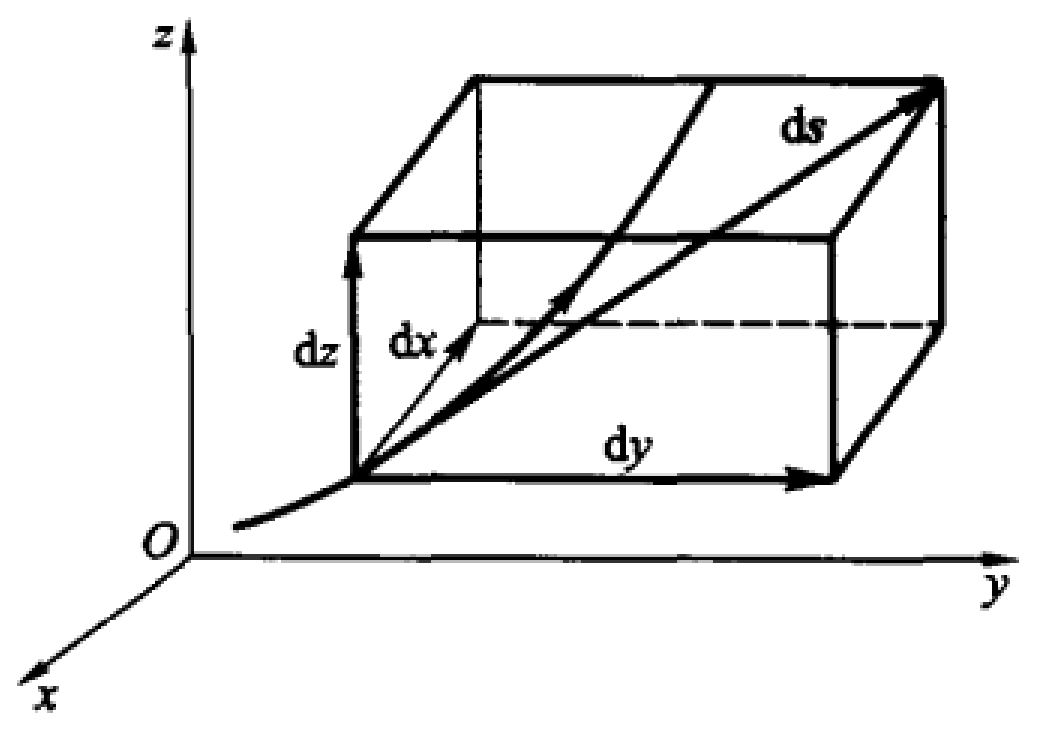
\includegraphics[width=0.5\textwidth]{work/figures/fig21-8}\caption{\relax}\label{fig:21-8}
\end{figure}

特别地，当 $\widehat{AB}$ 是平面曲线时，$\cos(\bm{\tau},z)=0$，则有
\[
\int_{\widehat{AB}}P\,\mathrm{d}x+Q\,\mathrm{d}y=\int_{\widehat{AB}}\left[P\cos(\bm{\tau},x)+Q\cos(\bm{\tau},y)\right]\mathrm{d}s.
\]

\begin{example}\label{ex:21-3-3}
求 $\displaystyle\oint_{L}\frac{x\,\mathrm{d}x+y\,\mathrm{d}y}{x^{2}+y^{2}}$，其中 $L$ 是 $x^{2}+y^{2}=a^{2}$ 沿逆时针方向．
\end{example}

\begin{proof}[解]
令
\[
\bm{F}=(P,Q)=\left(\frac{x}{x^{2}+y^{2}},\frac{y}{x^{2}+y^{2}}\right)=\frac{\bm{r}}{r^{2}},
\]
其中 $\bm{r}=\left\{x,y\right\}$ 是 $L$ 上点的向径，由于圆上每点的切线垂直于向径 $\bm{r}$，即 $\bm{r}\cdot\bm{\tau}=0$，因此由两种曲线积分的联系得
\[
\int_{L}\frac{x\,\mathrm{d}x+y\,\mathrm{d}y}{x^{2}+y^{2}}=\int_{L}\frac{1}{a^{2}}\bm{r}\cdot\bm{\tau}\,\mathrm{d}s=0.
\]
\end{proof}

\begin{figure}[htbp]
\centering
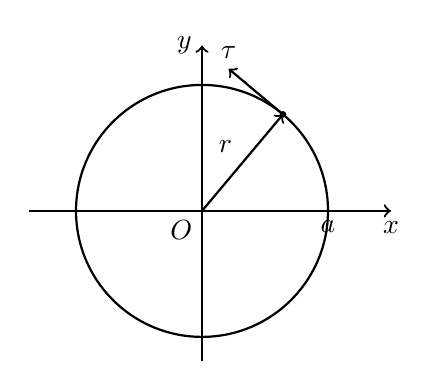
\begin{tikzpicture}[scale=1]
\draw[->,thick] (-2.2,0) -- (2.4,0) node[below] {$x$};
\draw[->,thick] (0,-1.9) -- (0,2.1) node[left] {$y$};
\draw[thick] (0,0) circle (1.6);
\draw[->,thick] (0,0) -- (50:1.6) node[midway,above left] {$\bm{r}$};
\fill (50:1.6) circle (1.2pt);
\draw[->,thick] (50:1.6) -- ++(140:0.9) node[above] {$\bm{\tau}$};
\node[below left] at (0,0) {$O$};
\node[below] at (1.6,0) {$a$};
\end{tikzpicture}\caption{\relax}\label{fig:21-9}
\end{figure}

\subsection{流量与第二型曲面积分}

先从一个物理问题谈起．

设空间有一块流体．如果对于空间区域 $V$ 的每一点 $(x,y,z)$ 与每一时刻 $t$，都对应一个流体的速度向量 $\bm{v}(x,y,z,t)$，那么就称流体在 $V$ 确定了一个速度的向量场 $\bm{v}(x,y,z,t)$．用数学的语言说，一个速度向量场就是一个定义在空间某区域 $V$ 上的向量值函数，另外，它可能还依赖于参数——时间 $t$．在研究江河海洋的水流运动中，在研究大气的运动中（天气预报、台风预报等），在研究爆炸过程激波的产生与运动中，速度场是常见的一个量．如果速度场不依赖于 $t$，即 $\bm{v}$ 仅是 $x$，$y$，$z$ 的函数，则称速度场是\emph{定常}的；如果速度场不仅依赖于 $x$，$y$，$z$ 还依赖于时间 $t$，则称速度场是\emph{不定常}的．研究工作总是从简单到复杂，因此，人们首先研究定常的速度场．一个最简单的物理问题是，设在一定常的速度场的定义域内，有一光滑的曲面 $S$，我们问，单位时间流过 $S$ 的流体是多少？如何计算？也就是说，如何计算流体通过 $S$ 的流量．

为解决这个问题，首先遇到的问题是，什么叫做流过（或通过）？直观的理解是从曲面的一侧到曲面的另一侧．然则什么叫曲面的侧？曲面永远都有两侧吗？

先假设 $S$ 不是闭曲面，这时它的边缘由逐段光滑的曲线 $L$ 构成．由于曲面 $S$ 是光滑的，因此在 $S$ 的每一点 $M$ 都有切平面，且切平面的位置随切点的位置而连续地变动．自然，在 $S$ 的每一点 $M$ 也有两个相反方向的单位法向量，它们是否分别代表了曲面在 $M$ 点的两侧？问题在于什么是曲面的侧．由于曲面 $S$ 是光滑的，曲面上两点 $M_{1}$ 与 $M_{2}$，它们上面分别有取定方向的两个法向量 $\bm{n}_{1}$，$\bm{n}_{2}$．如果在曲面上沿光滑曲线 $\Gamma$ 由 $M_{1}$ 运动到 $M_{2}$，则法向量 $\bm{n}_{1}$ 连续地变化．当它变到 $M_{2}$ 时，若法向量与 $\bm{n}_{2}$ 同向，自然便认为 $\bm{n}_{1}$ 与 $\bm{n}_{2}$ 是在曲面的同侧（图~\ref{fig:21-10}）；若 $\bm{n}_{1}$ 连续运动至 $M_{2}$ 时的法向量与 $\bm{n}_{2}$ 反向，自然便认为 $\bm{n}_{1}$ 与 $\bm{n}_{2}$ 是在曲面的异侧．因此，在曲面上取定点 $M_{1}$，在 $M_{1}$ 取定一法向量 $\bm{n}_{1}$，则由 $M_{1}$ 沿 $S$ 的光滑曲线而不越过 $S$ 的边缘，连续地走遍 $S$，便得到了 $S$ 中与 $\bm{n}_{1}$ 同侧的全体法向量．通常，人们会认为，对与 $\bm{n}_{1}$ 反向的 $-\bm{n}_{1}$，用同样的办法，即由 $M_{1}$ 出发沿 $S$ 的光滑曲线而不越过曲面的边缘，连续地走遍 $S$，便得到了 $S$ 中与 $-\bm{n}_{1}$ 同向的全体法向量．这样，便把曲面的两侧区分开来了．

\begin{figure}[htbp]
\centering
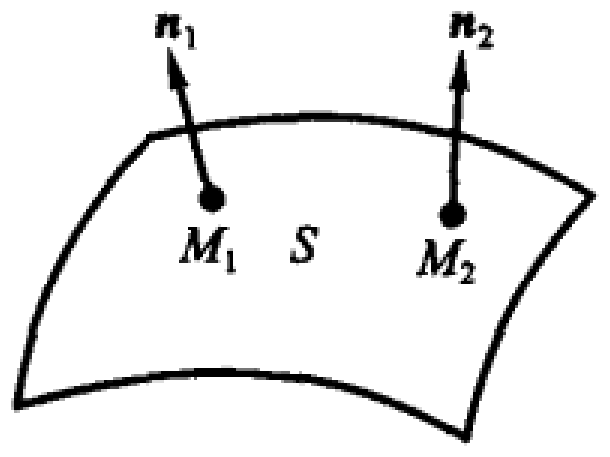
\includegraphics[width=0.4\textwidth]{work/figures/fig21-10}\caption{\relax}\label{fig:21-10}
\end{figure}

现在，问题在于，从 $M_{1}$ 出发，$\bm{n}_{1}$ 沿 $S$ 的光滑曲线而不越过曲面的边缘连续地变化，是否可能回到 $M_{1}$ 时变成了 $-\bm{n}_{1}$？也就是说，$\bm{n}_{1}$ 与 $-\bm{n}_{1}$ 可能在曲面的同一侧．换句话说，是否存在曲面，它不是双侧的而是单侧的．所谓\emph{默比乌斯}（Möbius，A.F.，1790—1868）带就是这种单侧曲面的曲型例子．将长方形纸条 $ABCD$ 先扭转一次，然后使 $B$ 与 $D$ 及 $A$ 与 $C$ 粘合起来（图~\ref{fig:21-11}），构成一条非闭的环带，便是默比乌斯带了．它的确具有上述单侧曲面的性质．假如用一种颜色涂这条环带，则可以不越过边缘而涂遍它的全部．对单侧曲面，自然不便说流体``通过''它的流量，因此，本书以后只讨论双侧曲面，除特别说明外，曲面都是指双侧的．

\begin{figure}[htbp]
\centering
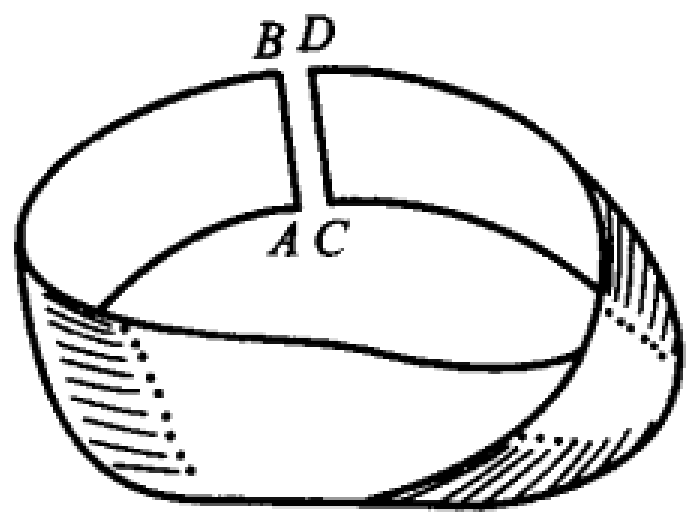
\includegraphics[width=0.4\textwidth]{work/figures/fig21-11}\caption{\relax}\label{fig:21-11}
\end{figure}

设 $S$ 是一双侧曲面，根据上面对曲面的侧的描述，如果在 $S$ 上任一点 $M_{1}$ 的法线上选定了一个确定的方向，则曲面上全部点的同侧法线也随之确定，也就是选定了曲面的一侧；如果原先选定的法线方向改变，则在其它点的法线方向也一律改变，这样就确定了曲面的另一侧．故对双侧曲面要确定它的一侧，只要在它上面任一点确定一法线方向就行了．

下面研究实际上怎样确定曲面的侧．设光滑曲面由函数
\[
z=f(x,y),\ (x,y)\in D
\]
确定，其中 $f(x,y)$ 在 $D$ 有连续的偏导数
\[
p=\frac{\partial f}{\partial x},\quad q=\frac{\partial f}{\partial y}.
\]
这样，曲面在每一点都有切平面，从而在每一点都有确定的法线．由第十六章 §3 知，曲面 $S$ 的单位法向量为
\[
\begin{aligned}
&\left(\cos\alpha,\cos\beta,\cos\gamma\right)\\
={}&\left(\frac{-p}{\pm\sqrt{1+p^{2}+q^{2}}},\frac{-q}{\pm\sqrt{1+p^{2}+q^{2}}},\frac{1}{\pm\sqrt{1+p^{2}+q^{2}}}\right).
\end{aligned}
\]
可见只要取定根式前正负号，三个分量都是 $x$，$y$ 的连续函数，也就是说法线的方向是随点的位置而连续变动的．因此，根式前正负号的选择，便表示确定了曲面的一侧．例如，若选取正号，则 $\cos\gamma>0$，它表示法向与 $z$ 轴正向交角为锐角，这就是通常所说的曲面的上侧．若选取负号，则所确定的一侧是曲面的下侧．这时法线与 $z$ 轴正向的交角是钝角．

设光滑曲面由参数方程
\[
x=x(u,v),\quad y=y(u,v),\quad z=z(u,v),\quad(u,v)\in\Delta
\]
给出．记
\[
A=\frac{\partial(y,z)}{\partial(u,v)},\quad B=\frac{\partial(z,x)}{\partial(u,v)},\quad C=\frac{\partial(x,y)}{\partial(u,v)}.
\]
由曲面光滑知 $A^{2}+B^{2}+C^{2}\neq0$，这时曲面 $S$ 上的单位法向量为
\[
\bm{n}=\left(\frac{A}{\pm\sqrt{A^{2}+B^{2}+C^{2}}},\frac{B}{\pm\sqrt{A^{2}+B^{2}+C^{2}}},\frac{C}{\pm\sqrt{A^{2}+B^{2}+C^{2}}}\right).
\]
只要取定根式前的正负号，则三个分量都是 $u$，$v$ 的连续函数，也就是说法线的方向随点的位置而连续移动．这样，如果选正号，则表示选定了曲面的一侧，如果选负号，则表示选定了曲面的另一侧．至于正号对应于曲面的哪一侧，只要选一点计算出 $\bm{n}$，再在图形上把 $\bm{n}$ 表示出来，便知道正号对应的是哪一侧．

对于封闭曲面，通常把两侧分为内侧和外侧，即法向量指向曲面所围立体的内部的一侧为内侧，而另一侧为外侧．例如球面 $x^{2}+y^{2}+z^{2}=R^{2}$ 的内侧，对上半球面 $(z>0)$ 是下侧，而对下半球面 $(z<0)$ 是上侧．容易看出，无论是内侧或外侧，单位法向量是随着点在球面上移动而连续变化的．

现在我们可以计算流体的速度场为 $\bm{v}(x,y,z)$ 时的流量问题了．设 $S$ 是双侧曲面，取定一侧为正侧，这时对应的单位法向量 $\bm{n}=(\cos\alpha,\cos\beta,\cos\gamma)$ 的每一个分量都是曲面上点 $(x,y,z)$ 的连续函数．设
\[
\bm{v}(x,y,z)=\left(P(x,y,z),Q(x,y,z),R(x,y,z)\right),
\]
其中 $P$，$Q$，$R$ 在 $S$ 上连续．我们要求流体在单位时间内从 $S$ 的负侧流向正侧的流量．

任给 $S$ 一个分法 $\Delta S_{i}$ $(i=1,2,\cdots,n)$，其面积仍记为 $\Delta S_{i}$．任取 $(\xi_{i},\eta_{i},\zeta_{i})\in\Delta S_{i}$，在这点的流速向量为 $\bm{v}(\xi_{i},\eta_{i},\zeta_{i})$，在这点的单位法向量为 $\bm{n}(\xi_{i},\eta_{i},\zeta_{i})$．当 $\Delta S_{i}$ 的直径很小时，可以把 $\Delta S_{i}$ 看成切平面上的一小块面积为 $\Delta S_{i}$ 的小区域，而在这小块区域内每点的流速是不变的，可取为 $\bm{v}(\xi_{i},\eta_{i},\zeta_{i})$．这样，单位时间流过 $\Delta S_{i}$ 的流体应该填满以 $\Delta S_{i}$ 为底，以 $\left|\bm{v}(\xi_{i},\eta_{i},\zeta_{i})\right|$ 为斜长的一个柱体（见图~\ref{fig:21-12}）．已知 $\Delta S_{i}$ 的法向量为 $\bm{n}(\xi_{i},\eta_{i},\zeta_{i})$，则不难看出，这个斜柱体的体积为
\[
\bm{v}(\xi_{i},\eta_{i},\zeta_{i})\Delta S_{i}\cdot\bm{n}(\xi_{i},\eta_{i},\zeta_{i}),
\]
也就是单位时间流过 $\Delta S_{i}$ 的流量．值得注意的是，这个量可正可负．如果是正的，这时 $\bm{v}$ 和 $\bm{n}$ 的交角是锐角，它表示流体由负侧流到正侧．如果是负的，这时 $\bm{v}$ 与 $\bm{n}$ 的交角是钝角，它表示流体由正侧流到负侧．但无论如何它的大小是单位时间流过 $\Delta S_{i}$ 的流量．因此单位时间流过整个 $S$ 的流量近似等于
\[
\sigma=\sum_{i=1}^{n}\bm{v}(\xi_{i},\eta_{i},\zeta_{i})\cdot\bm{n}(\xi_{i},\eta_{i},\zeta_{i})\Delta S_{i}.
\]
当 $\lambda=\max\limits_{1\leqslant i\leqslant n}\left\{d(\Delta S_{i})\right\}\to0$ 时（其中 $d(\Delta S_{i})$ 表示 $\Delta S_{i}$ 的直径），上述和式的极限便应该等于单位时间流过 $S$ 的流量．

\begin{figure}[htbp]
\centering
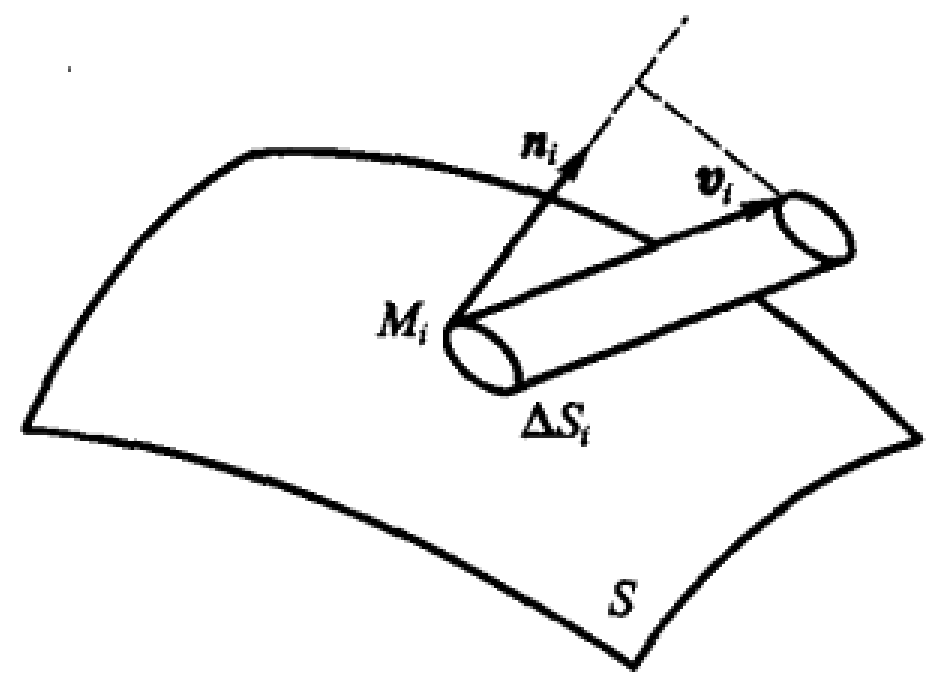
\includegraphics[width=0.5\textwidth]{work/figures/fig21-12}\caption{\relax}\label{fig:21-12}
\end{figure}

下面我们把和式 $\sigma$ 用分量表示出来．记
\[
\bm{n}(\xi_{i},\eta_{i},\zeta_{i})=\left(\cos\alpha_{i},\cos\beta_{i},\cos\gamma_{i}\right),
\]
则
\begin{align}
&\bm{v}(\xi_{i},\eta_{i},\zeta_{i})\cdot\bm{n}(\xi_{i},\eta_{i},\zeta_{i})\Delta S_{i}\notag\\
={}&P(\xi_{i},\eta_{i},\zeta_{i})\cos\alpha_{i}\Delta S_{i}+Q(\xi_{i},\eta_{i},\zeta_{i})\cos\beta_{i}\Delta S_{i}+\notag\\
&R(\xi_{i},\eta_{i},\zeta_{i})\cos\gamma_{i}\Delta S_{i}. \tag{3}\label{eq:21-2-3}
\end{align}
我们来看最后一项．注意，这里的 $\cos\gamma_{i}$ 是 $\bm{n}$ 与 $z$ 轴正向交角的余弦，因此可以把 $\Delta S_{i}\cos\gamma_{i}$ 看成 $\Delta S_{i}$ 在 $Oxy$ 平面投影的面积，当 $\cos\gamma_{i}>0$ 时，这面积取正号，当 $\cos\gamma_{i}<0$ 时，这面积取负号．我们称它为 $\Delta S_{i}$ 在 $Oxy$ 平面的\emph{有向投影}，而把这个和
\[
\sum_{i=1}^{n}R(\xi_{i},\eta_{i},\zeta_{i})\cos\gamma_{i}\Delta S_{i}
\]
的极限称为 $R(x,y,z)$ 在 $S$ 正侧的对 $x$，$y$ 的第二型曲面积分．

一般地，我们给出下面的定义．

\begin{definition}\label{def:21-4}
设函数 $f(x,y,z)$ 定义在光滑的双侧曲面 $S$ 上．给定 $S$ 的一侧，这等于指定了 $S$ 上每一点的单位法向量 $\bm{n}(x,y,z)=(\cos\alpha,\cos\beta,\cos\gamma)$．任给 $S$ 一个分法 $\Delta S_{i}$，$i=1,2,\cdots,n$，其中 $\Delta S_{i}$ 既表示小块曲面，也表示曲面的面积．在 $\Delta S_{i}$ 中任取 $(\xi_{i},\eta_{i},\zeta_{i})$，记 $\Delta D_{i}$ 为 $\Delta S_{i}$ 在 $Oxy$ 平面的有向投影，即 $\Delta D_{i}=\Delta S_{i}\cos\gamma_{i}$，其中 $\cos\gamma_{i}$ 是 $\cos\gamma$ 在 $(\xi_{i},\eta_{i},\zeta_{i})$ 点的值．作和
\[
\sum_{i=1}^{n}f(\xi_{i},\eta_{i},\zeta_{i})\Delta D_{i}.
\]
若当 $\lambda=\max\limits_{1\leqslant i\leqslant n}\left(\mathrm{d}(\Delta S_{i})\right)\to0$ 时，上述和式的极限存在，则称这极限为 $f$ 在曲面指定侧对 $x$，$y$ 的\emph{第二型曲面积分}，记为
\[
\iint_{S}f(x,y,z)\,\mathrm{d}x\mathrm{d}y.
\]
总起来，就是
\[
\iint_{S}f(x,y,z)\,\mathrm{d}x\mathrm{d}y=\lim_{\lambda\to0}\sum_{i=1}^{n}f(\xi_{i},\eta_{i},\zeta_{i})\Delta D_{i}.
\]
\end{definition}

把 $\Delta S_{i}$ 投影到 $Oyz$ 平面和 $Ozx$ 平面，便可得到两个类似的第二型曲面积分
\[
\iint_{S}f(x,y,z)\,\mathrm{d}y\mathrm{d}z\quad\text{或}\quad\iint_{S}f(x,y,z)\,\mathrm{d}z\mathrm{d}x.
\]
根据上述定义，我们知道，流量等于三个第二型曲面积分之和
\[
\iint_{S}P(x,y,z)\,\mathrm{d}y\mathrm{d}z+Q(x,y,z)\,\mathrm{d}z\mathrm{d}x+R(x,y,z)\,\mathrm{d}x\mathrm{d}y.
\]
这三个积分联在一起的情形是经常会碰到的．值得指出的是，在这个积分号中没有标明在 $S$ 的哪一侧积分．因此，每次出现这种积分时，都要附带说明积分是对曲面的哪一侧进行的．现在我们看到了，所谓曲面的方向，在第二型曲面积分中，实际上指的是双侧曲面的侧．

从定义中易见，对同一曲面，不同侧的积分仅相差一个负号，即
\[
\iint\limits_{S\text{正侧}}P\,\mathrm{d}y\mathrm{d}z+Q\,\mathrm{d}z\mathrm{d}x+R\,\mathrm{d}x\mathrm{d}y=-\iint\limits_{S\text{负侧}}P\,\mathrm{d}y\mathrm{d}z+Q\,\mathrm{d}z\mathrm{d}x+R\,\mathrm{d}x\mathrm{d}y.
\]
若 $S$ 是母线平行于 $z$ 轴的柱面，则 $S$ 在 $Oxy$ 面上的投影为 $0$，因此恒有
\[
\iint_{S}f(x,y,z)\,\mathrm{d}x\mathrm{d}y=0.
\]
两种曲面积分的根本区别在于第一型曲面积分，曲面是无向的，而第二型曲面积分，曲面是有向的，是对指定的一侧进行的．然而两者也是有联系的．事实上，按定义~\ref{def:21-4}，在等式\eqref{eq:21-2-3}中，当 $\lambda\to0$，和式的极限应该是
\[
\iint_{S}P(x,y,z)\,\mathrm{d}y\mathrm{d}z+Q(x,y,z)\,\mathrm{d}z\mathrm{d}x+R(x,y,z)\,\mathrm{d}x\mathrm{d}y,
\]
而按照定义~\ref{def:21-2}，和式的极限也等于
\[
\iint_{S}\left(P(x,y,z)\cos\alpha+Q(x,y,z)\cos\beta+R(x,y,z)\cos\gamma\right)\mathrm{d}S.
\]
因此
\[
\iint_{S}P\,\mathrm{d}y\mathrm{d}z+Q\,\mathrm{d}z\mathrm{d}x+R\,\mathrm{d}x\mathrm{d}y=\iint_{S}\left(P\cos\alpha+Q\cos\beta+R\cos\gamma\right)\mathrm{d}S.
\]
这就是两型曲面积分的联系，左边是第二型曲面积分，右边是第一型曲面积分，其中 $(\cos\alpha,\allowbreak\cos\beta,\allowbreak\cos\gamma)$ 是 $S$ 在点 $(x,y,z)$ 对应于左边积分 $S$ 那一侧的单位法向量．同曲线积分类似，当积分换成在 $S$ 的另一侧进行时，等式左边多一个负号．等式右边因是第一型曲面积分，应与曲面的侧无关，但这时法线换了一个方向，即每一点单位法向量 $(\cos\alpha,\allowbreak\cos\beta,\allowbreak\cos\gamma)$ 都变了符号，因此积分后仍然相等．

上式把第二型曲面积分化成了第一型曲面积分，而第一型曲面积分我们已经会计算了．因此，原则上已解决了第二型曲面积分的计算问题．但这样计算有时很繁．下面的定理表明，可以直接把第二型曲面积分化为二重积分进行计算．

\begin{theorem}\label{thm:21-4}
设 $R(x,y,z)$ 在光滑曲面
\[
S:\ z=z(x,y),\ (x,y)\in D
\]
上连续，则
\[
\iint_{S}R(x,y,z)\,\mathrm{d}x\mathrm{d}y=\pm\iint_{D}R(x,y,z(x,y))\,\mathrm{d}x\mathrm{d}y,
\]
其中 $S$ 为上侧时取正号，$S$ 为下侧时取负号．
\end{theorem}

\begin{proof}
沿用定义~\ref{def:21-4} 中的记号
\[
\begin{aligned}
\iint_{S}R(x,y,z)\,\mathrm{d}x\mathrm{d}y&=\lim_{\lambda\to0}\sum_{i=1}^{n}R(\xi_{i},\eta_{i},\zeta_{i})\Delta D_{i}\\
&=\lim_{\lambda\to0}\Big(\pm\sum_{i=1}^{n}R\big(\xi_{i},\eta_{i},z(\xi_{i},\eta_{i})\big)\big|\Delta D_{i}\big|\Big),
\end{aligned}
\]
其中 $S$ 为上侧时取正号，$S$ 为下侧时取负号．这时极限号下是二元函数的黎曼和，记 $\lambda'=\max\limits_{1\leqslant i\leqslant n}\{\Delta D_{i}\ \text{的直径}\}$，则有 $\lambda\to0$ 当且仅当 $\lambda'\to0$．又由 $R(x,y,z(x,y))$ 在 $D$ 连续，从而可积，于是由二重积分的定义即得
\[
\begin{aligned}
&\iint_{S}R(x,y,z)\,\mathrm{d}x\mathrm{d}y\\
={}&\lim_{\lambda'\to0}\pm\sum_{i=1}^{n}R\big(\xi_{i},\eta_{i},z(\xi_{i},\eta_{i})\big)\big|\Delta D_{i}\big|\\
={}&\pm\iint_{D}R\big(x,y,z(x,y)\big)\,\mathrm{d}x\mathrm{d}y.
\end{aligned}
\]
定理~\ref{thm:21-4} 证完．
\end{proof}

类似地可以证明，在相应条件下有
\[
\iint_{S}P(x,y,z)\,\mathrm{d}y\mathrm{d}z=\pm\iint_{E}P(x(y,z),y,z)\,\mathrm{d}y\mathrm{d}z,
\]
其中 $S$ 是前侧时取正号，$S$ 是后侧时取负号，$E$ 是 $S$ 在 $Oyz$ 平面的投影；
\[
\iint_{S}Q(x,y,z)\,\mathrm{d}z\mathrm{d}x=\pm\iint_{G}Q(x,y(x,z),z)\,\mathrm{d}z\mathrm{d}x,
\]
其中 $S$ 是右侧时取正号，$S$ 是左侧时取负号，$G$ 是 $S$ 在 $Ozx$ 平面的投影．

定理~\ref{thm:21-4} 中的公式对分片光滑曲面 $S$ 仍成立，因为这时沿曲面 $S$ 的积分等于有限块光滑曲面的积分之和．

\begin{example}\label{ex:21-4-1}
计算 $I=\displaystyle\iint_{S}x\,\mathrm{d}y\mathrm{d}z+y\,\mathrm{d}z\mathrm{d}x+z\,\mathrm{d}x\mathrm{d}y$，其中 $S$ 是顶点为 $(1,0,0)$，$(0,1,0)$，$(0,0,1)$ 的三角形的下侧．
\end{example}

\begin{figure}[htbp]
\centering
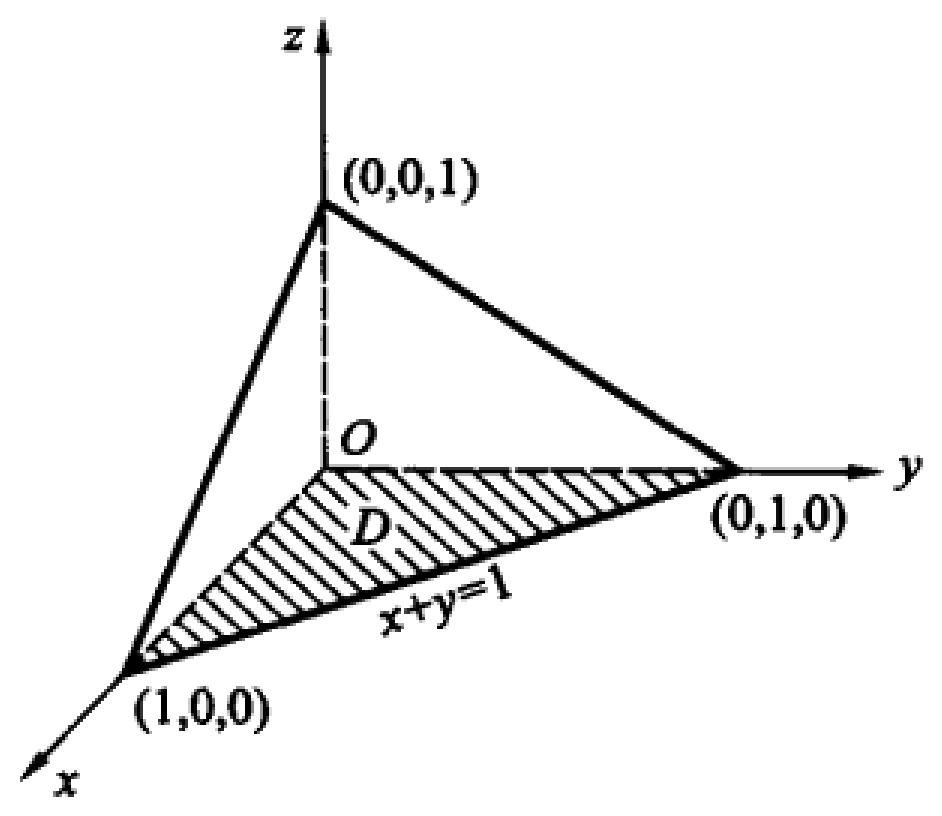
\includegraphics[width=0.5\textwidth]{work/figures/fig21-13}\caption{\relax}\label{fig:21-13}
\end{figure}

\begin{proof}[解法1]
曲面 $S$ 的方程为 $x+y+z=1$，它在 $xy$ 面上的投影为 $D$，由积分表达式的对称性及 $S$ 的对称性，有
\[
\begin{aligned}
I&=3\iint_{S}z\,\mathrm{d}x\mathrm{d}y=-3\iint_{D}(1-x-y)\,\mathrm{d}x\mathrm{d}y\\
&=-3\int_{0}^{1}\mathrm{d}x\int_{0}^{1-x}(1-x-y)\,\mathrm{d}y=-\frac{1}{2}.
\end{aligned}
\]
\end{proof}

\begin{proof}[解法2]
利用两种曲面积分的关系．因为曲面为 $x+y+z=1$ 的下侧，所以
\[
\bm{n}=-\frac{1}{\sqrt{3}}\{1,1,1\},
\]
\[
\begin{aligned}
I&=\iint_{S}x\,\mathrm{d}y\mathrm{d}z+y\,\mathrm{d}z\mathrm{d}x+z\,\mathrm{d}x\mathrm{d}y\\
&=-\frac{1}{\sqrt{3}}\iint_{S}(x+y+z)\,\mathrm{d}S=-\frac{1}{\sqrt{3}}\iint_{S}\mathrm{d}S\\
&=-\frac{1}{\sqrt{3}}\cdot\frac{1}{2}\cdot\sqrt{2}\cdot\sqrt{2}\sin\frac{\pi}{3}=-\frac{1}{2}.
\end{aligned}
\]
\end{proof}

\begin{example}\label{ex:21-4-2}
计算 $I=\displaystyle\iint_{S}x^{2}\,\mathrm{d}y\mathrm{d}z+y^{2}\,\mathrm{d}z\mathrm{d}x+z^{2}\,\mathrm{d}x\mathrm{d}y$，其中 $S$ 是半球面 $x^{2}+y^{2}+z^{2}=1$ $(z\geqslant0)$ 的上侧．
\end{example}

\begin{proof}[解]
对于 $\displaystyle\iint_{S}x^{2}\,\mathrm{d}y\mathrm{d}z$，将 $S$ 分为 $S_{1}$ 和 $S_{2}$ 两部分：

$S_{1}:x^{2}+y^{2}+z^{2}=1$ $(z\geqslant0,x\geqslant0)$ 前侧，

$S_{2}:x^{2}+y^{2}+z^{2}=1$ $(z\geqslant0,x\leqslant0)$ 后侧，

$S_{1}$，$S_{2}$ 在 $Oyz$ 面上的无向投影都是 $D$，故
\[
\begin{aligned}
\iint_{S}x^{2}\,\mathrm{d}y\mathrm{d}z&=\iint_{S_{1}}x^{2}\,\mathrm{d}y\mathrm{d}z+\iint_{S_{2}}x^{2}\,\mathrm{d}y\mathrm{d}z\\
&=\iint_{D}\left(1-y^{2}-z^{2}\right)\mathrm{d}y\mathrm{d}z-\iint_{D}\left(1-y^{2}-z^{2}\right)\mathrm{d}y\mathrm{d}z=0.
\end{aligned}
\]
由对称性立即可知，$\displaystyle\iint_{S}y^{2}\,\mathrm{d}z\mathrm{d}x=0$，而
\[
\begin{aligned}
\iint_{S}z^{2}\,\mathrm{d}x\mathrm{d}y&=\iint_{x^{2}+y^{2}\leqslant1}(1-x^{2}-y^{2})\,\mathrm{d}x\mathrm{d}y\\
&=\int_{0}^{2\pi}\mathrm{d}\theta\int_{0}^{1}(1-r^{2})r\,\mathrm{d}r=\frac{\pi}{2}.
\end{aligned}
\]
所以 $I=\dfrac{\pi}{2}$．
\end{proof}

\begin{figure}[htbp]
\centering
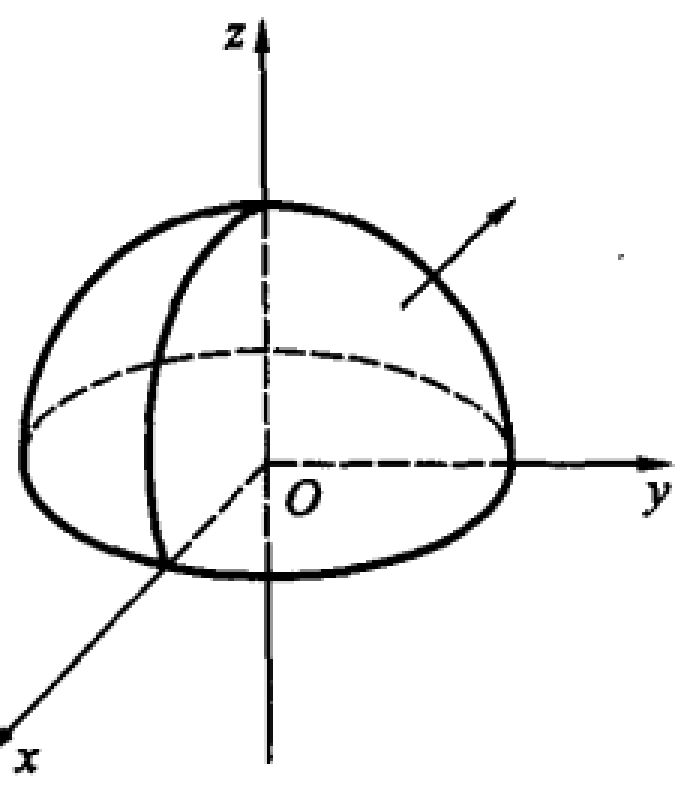
\includegraphics[width=0.45\textwidth]{work/figures/fig21-14}\caption{\relax}\label{fig:21-14}
\end{figure}

利用两种曲面积分之间的关系，我们立即可以导出 $S$ 由参数形式给出时的计算公式．设光滑曲面 $S$ 的参数方程为
\[
x=x(u,v),\quad y=y(u,v),\quad z=z(u,v),\quad(u,v)\in D
\]
则沿用前面的记号有
\[
\bm{n}=(\cos\alpha,\cos\beta,\cos\gamma)=\frac{\pm1}{\sqrt{A^{2}+B^{2}+C^{2}}}(A,B,C)
\]
因此
\[
\begin{aligned}
&\iint_{S}R(x,y,z)\,\mathrm{d}x\mathrm{d}y\\
={}&\iint_{S}R(x,y,z)\cos\gamma\,\mathrm{d}S\\
={}&\pm\iint_{D}R\big(x(u,v),y(u,v),z(u,v)\big)\,|C|\,\mathrm{d}u\mathrm{d}v\\
={}&\pm\iint_{D}R\big(x(u,v),y(u,v),z(u,v)\big)\left|\frac{\partial(x,y)}{\partial(u,v)}\right|\mathrm{d}u\mathrm{d}v,
\end{aligned}
\]
符号的选择为 $S$ 的上侧取正号，下侧取负号．

同理有
\[
\begin{aligned}
&\iint_{S}P(x,y,z)\,\mathrm{d}y\mathrm{d}z\\
={}&\pm\iint_{D}P\big(x(u,v),y(u,v),z(u,v)\big)\left|\frac{\partial(y,z)}{\partial(u,v)}\right|\mathrm{d}u\mathrm{d}v,
\end{aligned}
\]
符号的选择为 $S$ 的前侧取正号，后侧取负号．
\[
\begin{aligned}
&\iint_{S}Q(x,y,z)\,\mathrm{d}z\mathrm{d}x\\
={}&\pm\iint_{D}Q\big(x(u,v),y(u,v),z(u,v)\big)\left|\frac{\partial(z,x)}{\partial(u,v)}\right|\mathrm{d}u\mathrm{d}v,
\end{aligned}
\]
符号的选择为 $S$ 的右侧取正号，左侧取负号．

\begin{example}\label{ex:21-4-3}
求 $I=\displaystyle\iint_{S}x^{3}\,\mathrm{d}y\mathrm{d}z+y^{3}\,\mathrm{d}z\mathrm{d}x+z^{3}\,\mathrm{d}x\mathrm{d}y$，$S$ 是椭球面 $\dfrac{x^{2}}{a^{2}}+\dfrac{y^{2}}{b^{2}}+\dfrac{z^{2}}{c^{2}}=1$ 的外侧．
\end{example}

\begin{proof}[解]
$S$ 的参数方程为
\[
\begin{cases}
x=a\cos\theta\sin\varphi,\\
y=b\sin\theta\sin\varphi,\\
z=c\cos\varphi,
\end{cases}
\quad
\begin{aligned}
0&\leqslant\theta\leqslant2\pi,\\
0&\leqslant\varphi\leqslant\pi,
\end{aligned}
\]
\[
\frac{\partial(x,y)}{\partial(\varphi,\theta)}=\begin{vmatrix}a\cos\theta\cos\varphi&-a\sin\theta\sin\varphi\\ b\sin\theta\cos\varphi&b\cos\theta\sin\varphi\end{vmatrix}=ab\sin\varphi\cos\varphi.
\]
对于 $\displaystyle\iint_{S}z^{3}\,\mathrm{d}x\mathrm{d}y$，将 $S$ 分为上半椭球面 $S_{1}$ 的上侧和下半椭球面 $S_{2}$ 的下侧，则
\[
\begin{aligned}
&\iint_{S}z^{3}\,\mathrm{d}x\mathrm{d}y=\iint_{S_{1}}z^{3}\,\mathrm{d}x\mathrm{d}y+\iint_{S_{2}}z^{3}\,\mathrm{d}x\mathrm{d}y\\
&=\int_{0}^{2\pi}\mathrm{d}\theta\int_{0}^{\frac{\pi}{2}}(c\cos\varphi)^{3}\left|\frac{\partial(x,y)}{\partial(\varphi,\theta)}\right|\mathrm{d}\varphi-\int_{0}^{2\pi}\mathrm{d}\theta\int_{\frac{\pi}{2}}^{\pi}(c\cos\varphi)^{3}\left|\frac{\partial(x,y)}{\partial(\varphi,\theta)}\right|\mathrm{d}\varphi\\
&=2\pi abc^{3}\int_{0}^{\frac{\pi}{2}}\sin\varphi\cos^{4}\varphi\,\mathrm{d}\varphi+2\pi abc^{3}\int_{\frac{\pi}{2}}^{\pi}\cos^{4}\varphi\sin\varphi\,\mathrm{d}\varphi\\
&=4\pi abc^{3}\int_{0}^{\frac{\pi}{2}}\sin\varphi\cos^{4}\varphi\,\mathrm{d}\varphi=4\pi abc^{3}\,\frac{1}{5}\cos^{5}\varphi\,\Big|_{\frac{\pi}{2}}^{0}=\frac{4}{5}\pi abc^{3}.
\end{aligned}
\]
由对称性知
\[
\iint_{S}x^{3}\,\mathrm{d}y\mathrm{d}z=\frac{4}{5}\pi a^{3}bc,
\]
\[
\iint_{S}y^{3}\,\mathrm{d}z\mathrm{d}x=\frac{4}{5}\pi ab^{3}c,
\]
从而
\[
I=\frac{4}{5}\pi abc\left(a^{2}+b^{2}+c^{2}\right).
\]
\end{proof}

和第二型曲线积分类似，引入向量
\[
\begin{aligned}
\bm{F}(x,y,z)&=\left(P(x,y,z),Q(x,y,z),R(x,y,z)\right),\\
\mathrm{d}\bm{S}&=\bm{n}\cdot\mathrm{d}S=\left\{\cos\alpha,\cos\beta,\cos\gamma\right\}\mathrm{d}S\\
&=\left\{\mathrm{d}y\mathrm{d}z,\mathrm{d}z\mathrm{d}x,\mathrm{d}x\mathrm{d}y\right\},
\end{aligned}
\]
则
\[
\begin{aligned}
&\iint_{S}P\,\mathrm{d}y\mathrm{d}z+Q\,\mathrm{d}z\mathrm{d}x+R\,\mathrm{d}x\mathrm{d}y\\
={}&\iint_{S}\left(P\cos\alpha+Q\cos\beta+R\cos\gamma\right)\mathrm{d}S\\
={}&\iint_{S}\bm{F}\cdot\mathrm{d}\bm{S}.
\end{aligned}
\]
和曲线情形不同的是，这里 $\mathrm{d}\bm{S}$ 的方向为法线方向，与积分曲面 $S$ 的侧相同．

\begin{xiti}
\item 计算下列第二型曲线积分：
\begin{ziti}
\item $\displaystyle\int_{L}(2a-y)\,\mathrm{d}x+\mathrm{d}y$，其中 $L$ 为摆线 $x=a(t-\sin t)$，$y=a(1-\cos t)$ $(0\leqslant t\leqslant2\pi)$ 沿 $t$ 增加的方向；
\item $\displaystyle\int_{L}\dfrac{-x\,\mathrm{d}x+y\,\mathrm{d}y}{x^{2}+y^{2}}$，其中 $L$ 为圆周 $x^{2}+y^{2}=a^{2}$ 依逆时针方向；
\item $\displaystyle\int_{L}x\,\mathrm{d}x+y\,\mathrm{d}y+z\,\mathrm{d}z$，其中 $L$ 为从 $(1,1,1)$ 到 $(2,3,4)$ 的直线段；
\item $\displaystyle\int_{L}\left(x^{2}-2xy\right)\mathrm{d}x+\left(y^{2}-2xy\right)\mathrm{d}y$，$L$ 为 $y=x^{2}$ 从 $(1,1)$ 到 $(-1,1)$；
\item $\displaystyle\int_{L}y\,\mathrm{d}x-x\,\mathrm{d}y+\left(x^{2}+y^{2}\right)\mathrm{d}z$，$L$ 为曲线 $x=\mathrm{e}^{t}$，$y=\mathrm{e}^{-t}$，$z=at$ 从 $(1,1,0)$ 到 $\left(\mathrm{e},\mathrm{e}^{-1},a\right)$；
\item $\displaystyle\int_{L}\left(x^{2}+y^{2}\right)\mathrm{d}x+\left(x^{2}-y^{2}\right)\mathrm{d}y$，$L$ 为以 $A(1,0)$，$B(2,0)$，$C(2,1)$，$D(1,1)$ 为顶点的正方形沿逆时针方向．
\end{ziti}
\item 计算曲线积分
\[
\int_{L}\left(y^{2}-z^{2}\right)\mathrm{d}x+\left(z^{2}-x^{2}\right)\mathrm{d}y+\left(x^{2}-y^{2}\right)\mathrm{d}z.
\]
\begin{ziti}
\item $L$ 为球面三角形 $x^{2}+y^{2}+z^{2}=1$，$x\geqslant0$，$y\geqslant0$，$z\geqslant0$ 的边界线，从球的外侧看去，$L$ 的方向为逆时针方向；
\item $L$ 是球面 $x^{2}+y^{2}+z^{2}=a^{2}$ 和柱面 $x^{2}+y^{2}=ax$ $(a>0)$ 的交线位于 $Oxy$ 平面上方的部分，从 $x$ 轴上 $(b,0,0)$ $(b>a)$ 点看去，$L$ 是顺时针方向．
\end{ziti}
\item 求闭曲线 $L$ 上的第二型曲线积分
\[
\oint_{L}\dfrac{y\,\mathrm{d}x-x\,\mathrm{d}y}{x^{2}+y^{2}},
\]
\begin{ziti}
\item $L$ 为圆 $x^{2}+y^{2}=a^{2}$，逆时针方向；
\item $L$ 为椭圆 $\dfrac{x^{2}}{a^{2}}+\dfrac{y^{2}}{b^{2}}=1$，顺时针方向；
\item $L$ 为以 $(0,0)$ 为中心，边长为 $a$，对边平行于坐标轴的正方形，顺时针方向；
\item $L$ 是以 $(-1,-1)$，$(1,-1)$，$(0,1)$ 为顶点的三角形，顺时针方向．
\end{ziti}
\item 求力场 $\bm{F}$ 对运动的单位质点所作的功，此质点沿曲线 $L$ 从 $A$ 点运动到 $B$ 点：
\begin{ziti}
\item $\bm{F}=\left(x-2xy^{2},y-2x^{2}y\right)$，$L$ 为平面曲线 $y=x^{2}$，$A(0,0)$，$B(1,1)$；
\item $\bm{F}=(x+y,xy)$，$L$ 为平面曲线 $y=1-\left|1-x\right|$，$A(0,0)$，$B(2,0)$；
\item $\bm{F}=(x-y,y-z,z-x)$，$L$ 的矢量形式为 $\bm{r}(t)=t\bm{i}+t^{2}\bm{j}+t^{3}\bm{k}$，$A(0,0,0)$，$B(1,1,1)$；
\item $\bm{F}=\left(y^{2},z^{2},x^{2}\right)$，$L$ 的参数式为 $x=\alpha\cos t$，$y=\beta\sin t$，$z=\gamma t$ $(\alpha,\beta,\gamma$ 为正数)，$A(\alpha,0,0)$，$B(\alpha,0,2\pi\gamma)$．
\end{ziti}
\item 设 $P$，$Q$，$R$ 在 $L$ 上连续，$L$ 为光滑弧段，弧长为 $l$，证明
\[
\left|\int_{L}P\,\mathrm{d}x+Q\,\mathrm{d}y+R\,\mathrm{d}z\right|\leqslant Ml.
\]
其中 $M=\max\limits_{(x,y,z)\in L}\left\{\sqrt{P^{2}+Q^{2}+R^{2}}\right\}$．
\item 设光滑闭曲线 $L$ 在光滑曲面 $S$ 上，$S$ 的方程为 $z=f(x,y)$，曲线 $L$ 在 $Oxy$ 平面上的投影曲线为 $l$，函数 $P(x,y,z)$ 在 $L$ 上连续，证明：
\[
\oint_{L}P(x,y,z)\,\mathrm{d}x=\oint_{l}P(x,y,f(x,y))\,\mathrm{d}x.
\]
\item 计算 $I=\displaystyle\int_{L}xyz\,\mathrm{d}z$，其中 $L$ 为 $x^{2}+y^{2}+z^{2}=1$ 与 $y=z$ 相交的圆，其方向按曲线依次经过 $1$、$2$、$7$、$8$ 卦限．
\item 计算下列第二型曲面积分：
\begin{ziti}
\item $\displaystyle\iint_{S}y(x-z)\,\mathrm{d}y\mathrm{d}z+x^{2}\,\mathrm{d}z\mathrm{d}x+\left(y^{2}+xz\right)\mathrm{d}x\mathrm{d}y$，其中 $S$ 为 $x=y=z=0$，$x=y=z=a$ 六个平面所围的正立方体边界的外侧；
\item $\displaystyle\iint_{S}(x+y)\,\mathrm{d}y\mathrm{d}z+(y+z)\,\mathrm{d}z\mathrm{d}x+(z+x)\,\mathrm{d}x\mathrm{d}y$，其中 $S$ 是以原点为中心，边长为 $2$ 的正立方体表面的外侧；
\item $\displaystyle\iint_{S}yz\,\mathrm{d}z\mathrm{d}x$，$S$ 为 $\dfrac{x^{2}}{a^{2}}+\dfrac{y^{2}}{b^{2}}+\dfrac{z^{2}}{c^{2}}=1$ 的上半部分的上侧；
\item $\displaystyle\iint_{S}z\,\mathrm{d}x\mathrm{d}y+x\,\mathrm{d}y\mathrm{d}z+y\,\mathrm{d}z\mathrm{d}x$，$S$ 为柱面 $x^{2}+y^{2}=1$ 被平面 $z=0$ 及 $z=3$ 所截部分的外侧；
\item $\displaystyle\iint_{S}xy\,\mathrm{d}y\mathrm{d}z+yz\,\mathrm{d}z\mathrm{d}x+xz\,\mathrm{d}x\mathrm{d}y$，$S$ 是由平面 $x=y=z=0$ 和 $x+y+z=1$ 所围的四面体表面的外侧；
\item $\displaystyle\iint_{S}x^{3}\,\mathrm{d}y\mathrm{d}z+y^{3}\,\mathrm{d}z\mathrm{d}x+z^{3}\,\mathrm{d}x\mathrm{d}y$，$S$ 为球面 $x^{2}+y^{2}+z^{2}=a^{2}$ 的外侧；
\item $\displaystyle\iint_{S}x^{2}\,\mathrm{d}y\mathrm{d}z+y^{2}\,\mathrm{d}z\mathrm{d}x+z^{2}\,\mathrm{d}x\mathrm{d}y$，$S$ 是球面 $(x-a)^{2}+(y-b)^{2}+(z-c)^{2}=R^{2}$ 的外侧．
\end{ziti}
\item 设某流体的流速为 $\bm{v}=(k,y,0)$，求单位时间内从球面 $x^{2}+y^{2}+z^{2}=4$ 的内部流过球面的流量．
\item 设流体的流速为 $\bm{v}=\left(xy^{5},0,z^{5}x^{x}\right)$，求穿过柱面 $x^{2}+y^{2}=a^{2}$ $(-h\leqslant z\leqslant h)$ 外侧的流量．
\end{xiti}
